%
%Не забыть:
%--------------------------------------
%Вставить колонтитулы, поменять название на титульнике



%--------------------------------------

\documentclass[a4paper, 12pt]{article} 

%--------------------------------------
%Russian-specific packages
%--------------------------------------
%\usepackage[warn]{mathtext}
\usepackage[T2A]{fontenc}
\usepackage[utf8]{inputenc}
\usepackage[english,russian]{babel}
\usepackage[intlimits]{amsmath}
\usepackage{esint}
%--------------------------------------
%Hyphenation rules
%--------------------------------------
\usepackage{hyphenat}
\hyphenation{ма-те-ма-ти-ка вос-ста-нав-ли-вать}
%--------------------------------------
%Packages
%--------------------------------------
\usepackage{amsmath}
\usepackage{amssymb}
\usepackage{amsfonts}
\usepackage{amsthm}
\usepackage{latexsym}
\usepackage{mathtools}
\usepackage{etoolbox}%Булевые операторы
\usepackage{extsizes}%Выставление произвольного шрифта в \documentclass
\usepackage{geometry}%Разметка листа
\usepackage{indentfirst}
\usepackage{wrapfig}%Создание обтекаемых текстом объектов
\usepackage{fancyhdr}%Создание колонтитулов
\usepackage{setspace}%Настройка интерлиньяжа
\usepackage{lastpage}%Вывод номера последней страницы в документе, \lastpage
\usepackage{soul}%Изменение параметров начертания
\usepackage{hyperref}%Две строчки с настройкой гиперссылок внутри получаеммого
\usepackage[usenames,dvipsnames,svgnames,table,rgb]{xcolor}% pdf-документа
\usepackage{multicol}%Позволяет писать текст в несколько колонок
\usepackage{cite}%Работа с библиографией
\usepackage{subfigure}% Человеческая вставка нескольких картинок
\usepackage{tikz}%Рисование рисунков
\usepackage{float}% Возможность ставить H в положениях картинки
% Для картинок Моти
\usepackage{misccorr}
\usepackage{lscape}
\usepackage{cmap}



\usepackage{graphicx,xcolor}
\graphicspath{{Pictures/}}
\DeclareGraphicsExtensions{.pdf,.png,.jpg}

%----------------------------------------
%Список окружений
%----------------------------------------
\newenvironment {theor}[2]
{\smallskip \par \textbf{#1.} \textit{#2}  \par $\blacktriangleleft$}
{\flushright{$\blacktriangleright$} \medskip \par} %лемма/теорема с доказательством
\newenvironment {proofn}
{\par $\blacktriangleleft$}
{$\blacktriangleright$ \par} %доказательство
%----------------------------------------
%Список команд
%----------------------------------------
\newcommand{\grad}
{\mathop{\mathrm{grad}}\nolimits\,} %градиент

\newcommand{\diver}
{\mathop{\mathrm{div}}\nolimits\,} %дивергенция

\newcommand{\rot}
{\ensuremath{\mathrm{rot}}\,}

\newcommand{\Def}[1]
{\underline{\textbf{#1}}} %определение

\newcommand{\RN}[1]
{\MakeUppercase{\romannumeral #1}} %римские цифры

\newcommand {\theornp}[2]
{\textbf{#1.} \textit{ #2} \par} %Написание леммы/теоремы без доказательства

\newcommand{\qrq}
{\ensuremath{\quad \Rightarrow \quad}} %Человеческий знак следствия

\newcommand{\qlrq}
{\ensuremath{\quad \Leftrightarrow \quad}} %Человеческий знак равносильности

\renewcommand{\phi}{\varphi} %Нормальный знак фи

\newcommand{\me}
{\ensuremath{\mathbb{E}}}

\newcommand{\md}
{\ensuremath{\mathbb{D}}}



%\renewcommand{\vec}{\overline}




%----------------------------------------
%Разметка листа
%----------------------------------------
\geometry{top = 3cm}
\geometry{bottom = 2cm}
\geometry{left = 1.5cm}
\geometry{right = 1.5cm}
%----------------------------------------
%Колонтитулы
%----------------------------------------
\pagestyle{fancy}%Создание колонтитулов
\fancyhead{}
%\fancyfoot{}
%----------------------------------------
%Интерлиньяж (расстояния между строчками)
%----------------------------------------
%\onehalfspacing -- интерлиньяж 1.5
%\doublespacing -- интерлиньяж 2
%----------------------------------------
%Настройка гиперссылок
%----------------------------------------
\hypersetup{				% Гиперссылки
	unicode=true,           % русские буквы в раздела PDF
	pdftitle={Заголовок},   % Заголовок
	pdfauthor={Автор},      % Автор
	pdfsubject={Тема},      % Тема
	pdfcreator={Создатель}, % Создатель
	pdfproducer={Производитель}, % Производитель
	pdfkeywords={keyword1} {key2} {key3}, % Ключевые слова
	colorlinks=true,       	% false: ссылки в рамках; true: цветные ссылки
	linkcolor=blue,          % внутренние ссылки
	citecolor=blue,        % на библиографию
	filecolor=magenta,      % на файлы
	urlcolor=cyan           % на URL
}
%----------------------------------------
%Работа с библиографией (как бич)
%----------------------------------------
\renewcommand{\refname}{Список литературы}%Изменение названия списка литературы для article
%\renewcommand{\bibname}{Список литературы}%Изменение названия списка литературы для book и report
%----------------------------------------
\begin{document}
	\begin{titlepage}
		\begin{center}
			$$$$
			$$$$
			$$$$
			$$$$
			{\Large{НАЦИОНАЛЬНЫЙ ИССЛЕДОВАТЕЛЬСКИЙ УНИВЕРСИТЕТ}}\\
			\vspace{0.1cm}
			{\Large{ВЫСШАЯ ШКОЛА ЭКОНОМИКИ}}\\
			\vspace{0.25cm}
			{\large{Факультет физики}}\\
			\vspace{5.5cm}
			{\Huge\textbf{{Серия лабораторных работ по современной физике}}}\\%Общее название
			\vspace{1cm}
			{Работу выполнили студенты 3 курса}\\
			{Захаров Сергей Дмитриевич}\\
			{Еремин Валентин Антонович}\\
			{Святковская Ольга Алексеевна}\\
			\vfill
			
\includegraphics[width = 0.2\textwidth]{HSElogo}\\
			\vfill
			Москва\\
			2021
		\end{center}
	\end{titlepage}
	
\tableofcontents

\newpage

\section{Зависимость сопротивления материала от температуры}
\fancyhead[R]{\textsc{Зависимость сопротивления материала от температуры}}%Вставить колонтитул сюда

\subsection{Постановка целей работы}

\begin{enumerate}
	\item Сборка установки для изучения зависимости сопротивления образца от его температуры.
	
	\item Получение данных эксперимента.
	
	\item Анализ и интерпретация полученных данных.
\end{enumerate}

\subsection{Описание установки}

Для изучения зависимости $R(T)$ образца была предложена схема с использованием вольтметров, резистора, на который накручивалась проволока из изучаемого материала, платинового термометра (или термопары для серий с нагревом) и вспомогательного оборудования. Образцы погружался для охлаждения в жидкий азот, а также нагревался в кипящей воде. Электрическая схема эксперимента представлена на рисунке \ref{fig:1_scheme}.

\begin{figure}[H]
	\centering
	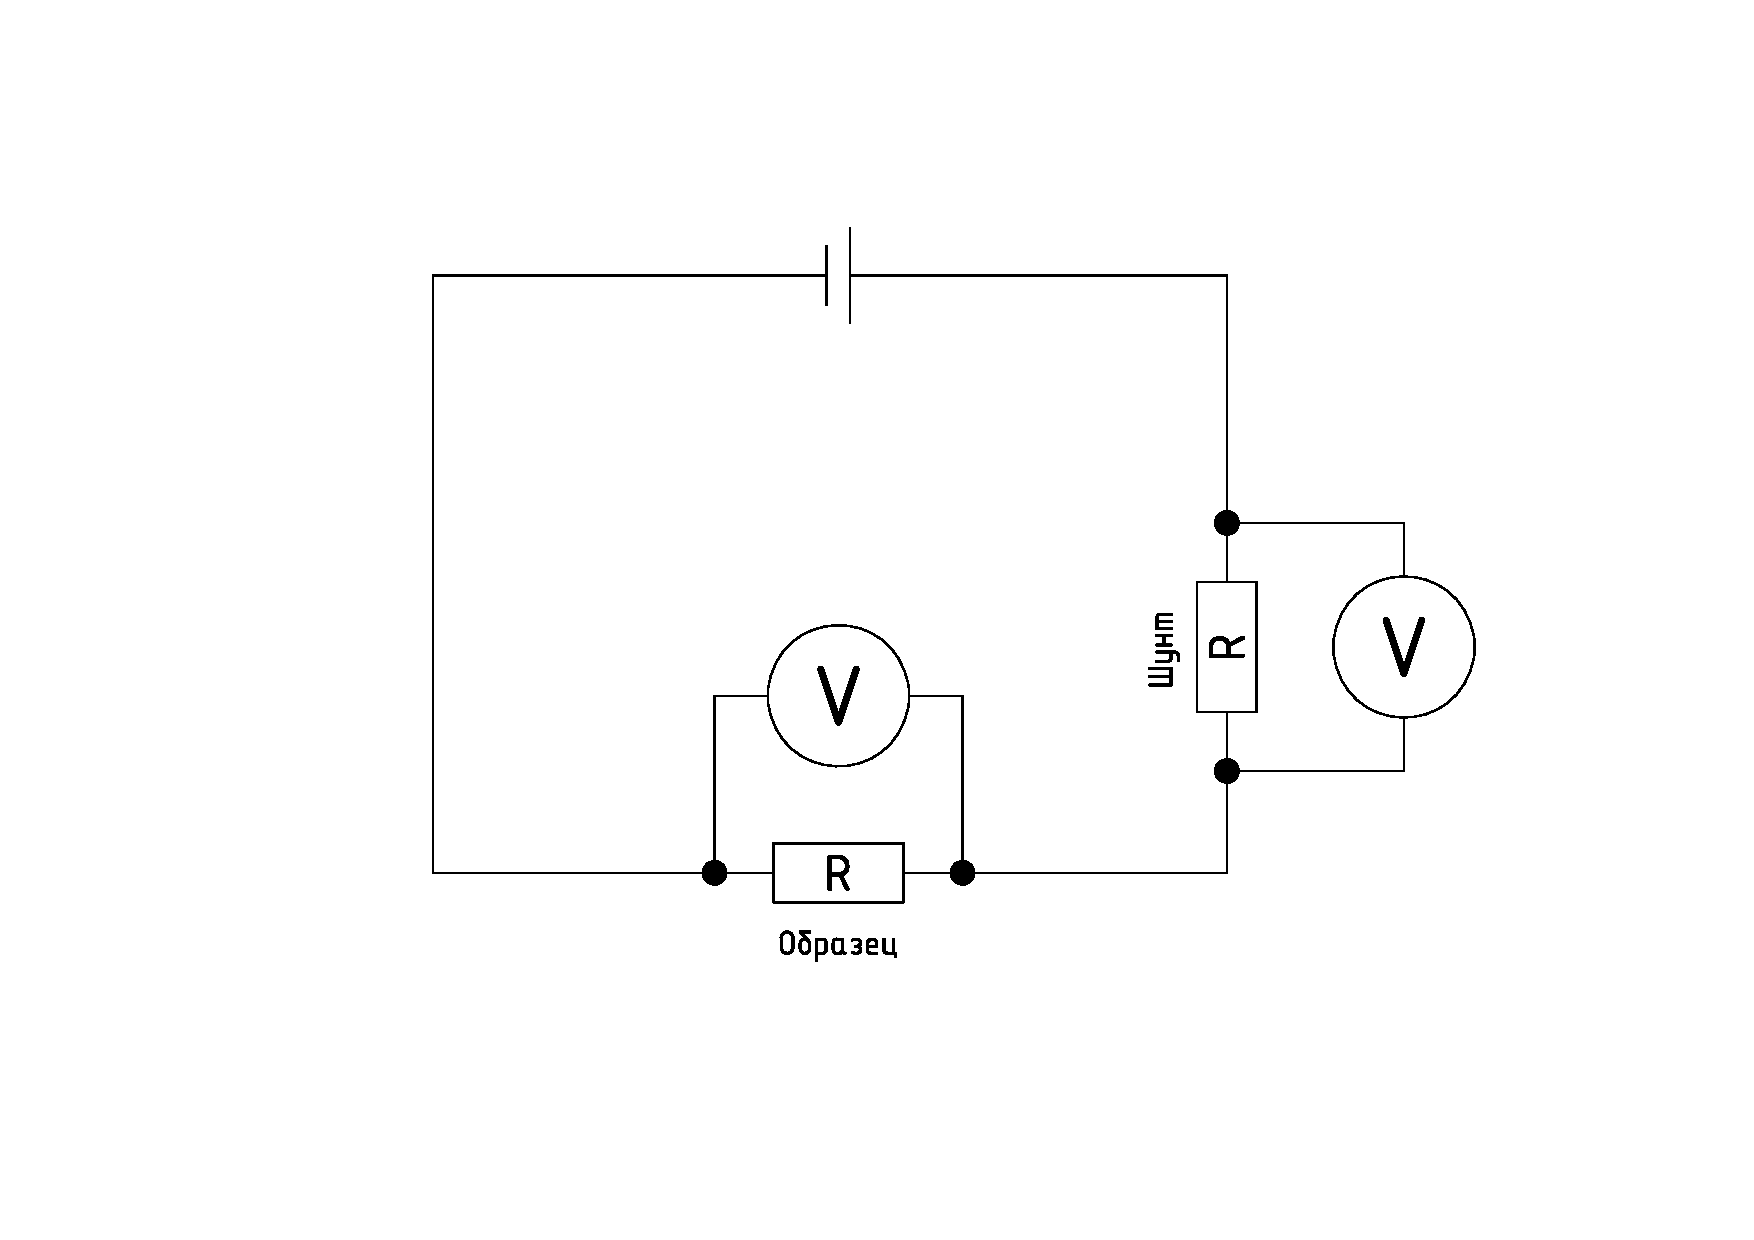
\includegraphics[width=\linewidth]{1_scheme}
	\caption{Электрическая схема для проведения эксперимента по получению температурных коэффициентов электрического сопротивления.}
	\label{fig:1_scheme}
\end{figure}

\subsection{Теоретическая база}

\subsubsection{Чистые металлы}

Колеблющийся атомы решетки могут рассматриваться как независимые беспорядочные центры рассеяния и поэтому вероятность рассеяния зависит от среднеквадратичной амплитуды решеточных колебаний $<\!X^2\!>$. Среднеквадратичная амплитуда гармонических колебаний пропорциональна температуре $T$. Таким образом, если пренебречь тепловым расширением, удельное сопротивление, как и сопротивление чистого металла в области высоких температур должно быть пропорционально $T$:

\begin{equation}
	\rho=\rho_0(1 + \alpha\Delta T )
	\label{eq:1_1}
\end{equation}

\subsubsection{Сплавы}
Введение значительного количества примесных атомов в твердый раствор приводит к искажению кристаллической решетки. Вследствие этого появляется дополнительный вклад в рассеяние. Рассеяние на статических дефектах структуры не зависит от температуры. Поэтому по мере приближения температуры к абсолютному нулю сопротивление реальных металлов стремится к некоторому постоянному значению, называемому остаточным сопротивлением, т.е. полное удельное сопротивление металла --- это сумма удельного сопротивления, обусловленного рассеянием электронов на тепловых колебаниях узлов кристаллической решетки, и остаточного удельного сопротивления, обусловленного рассеянием электронов на статических дефектов структуры.


Исключение из этого правила составляют сверхпроводящие металлы, в которых сопротивление исчезает ниже некоторой критической температуры.

Наиболее существенный вклад в остаточное сопротивление вносит рассеяние на примесях, которые всегда присутствуют в реальном проводнике либо в виде загрязнения, либо в виде легирующего (т.е. преднамеренно вводимого) элемента. Следует заметить, что любая примесная добавка приводит к повышению удельного сопротивления, даже если она обладает повышенной проводимостью по сравнению с основным металлом.

Итого, для определения температурных коэффициентов электрического сопротивления будем пользоваться следующей формулой, легко получаемой из \ref{eq:1_1}:

\begin{equation}
	\alpha(T_0) = \frac{1}{R(T_0)} \cdot \frac{d R}{d T}
\end{equation}

\subsection{Экспериментальные данные}

\subsubsection{Данные экспериментов при охлаждении}

Было проведено две серии экспериментов: по одному с охлаждением чистого металла (медь) и сплава (нихром) для определения температурной зависимости их сопротивления. Полученные зависимости представлены на рисунках \ref{fig:1_Cu_Cooling} (медь) и \ref{fig:1_Ni_Cooling} (нихром).

Из полученных графиков мы можем заключить, что зависимость сопротивления образца от температуры линейна для обоих образцов. Были также получены экспериментальные температурные коэффициенты электрического сопротивления для образцов при температуре 298 К, оказавшиеся равными:

\begin{align*}
	\alpha_{\text{Cu}} = 0.00452 \text{ К}^{-1}\\
	\alpha_{\text{Nic}} = 0.00017 \text{ К}^{-1}
\end{align*}

Полученные коэффициенты с хорошей точностью сходятся с табличными коэффициентами при той же температуре: $0.004 \text{ К}^{-1}$ для меди и $0.0002 \text{ К}^{-1}$ для нихрома.

\begin{figure}[H]
	\centering
	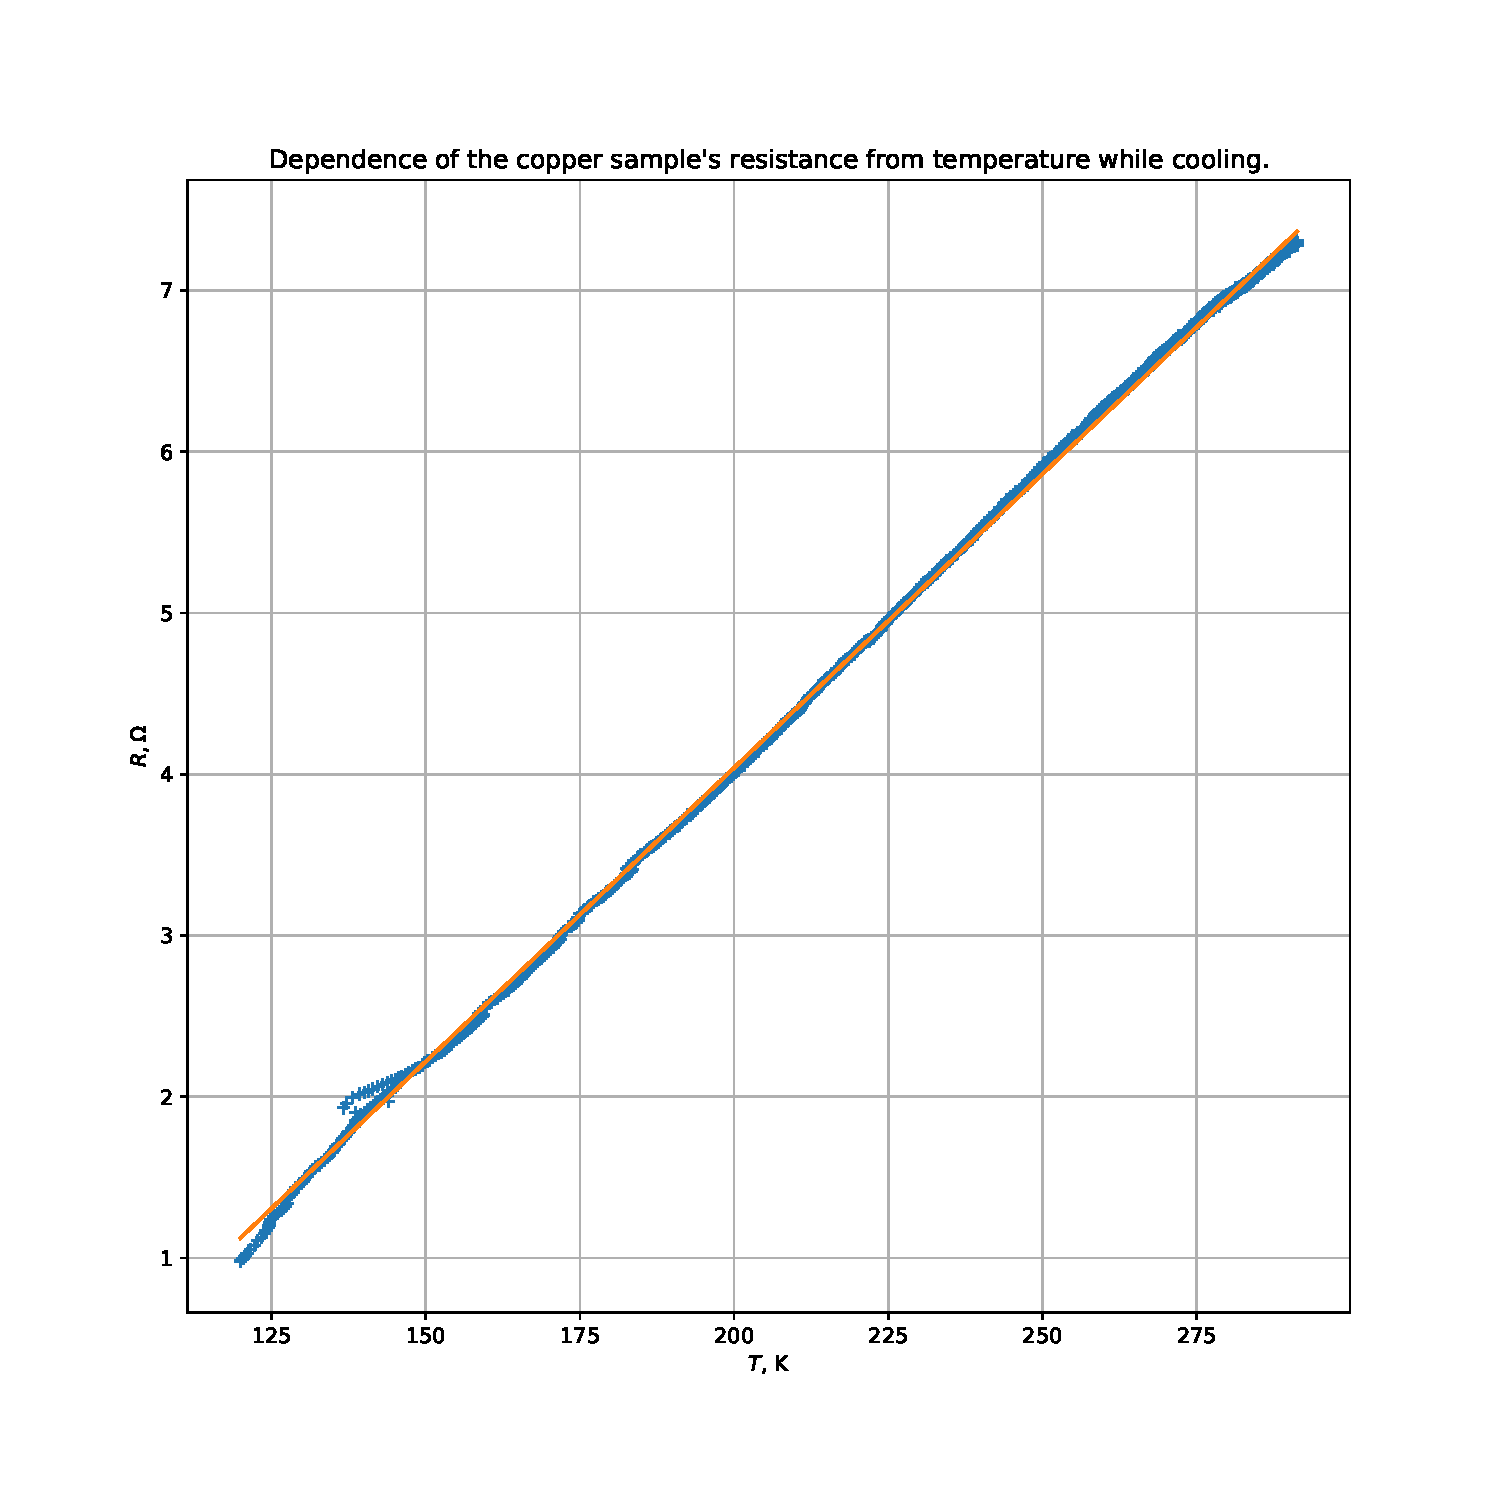
\includegraphics[width=\linewidth]{1_Cu_Cooling}
	\caption{Зависимость сопротивления образца меди от температуры при охлаждении с комнатной температуры до температуры, близкой к температуре жидкого азота.}
	\label{fig:1_Cu_Cooling}
\end{figure}

\begin{figure}[H]
	\centering
	\includegraphics[width=\linewidth]{1_Ni_Cooling}
	\caption{Зависимость сопротивления образца нихрома от температуры при охлаждении с комнатной температуры до температуры, близкой к температуре жидкого азота.}
	\label{fig:1_Ni_Cooling}
\end{figure}


\subsubsection{Данные экспериментов при высоких температурах}
Как и в предыдущем эксперименте, было проведено две серии экспериментов по одному с нагревом чистого металла (медь) и сплава (нихром) для определения температурной зависимости их сопротивления при теперь уже нагреве. Логичным ожидаемым результатом будет их корреляция с результатами прошлых серий.

При работе с медью возникла необходимость использования нового образца в связи с расплавкой лака на предыдущем образце.

При работе с медью параллельно проводилась калибровка термопары, из-за чего данные снимались вручную и точек получилось существенно меньше, чем при серии с нихромом.

Из представленных на рисунках \ref{fig:1_Cu_Heating} (медь) и \ref{fig:1_Ni_Heating} (нихром) данных видно, что зависимость в целом снова линейна. Сильная зашумленность данных с нихромом связана с тем, что само по себе изменение сопротивления у него крайне маленькое, из-за чего шумы оказываются порядка интересующей нас величины.

Также посмотрим на определенные в эксперименте температурные коэффициенты электрического сопротивления для образцов:

\begin{align*}
	\alpha_{\text{Cu}} = 0.00397 \text{ К}^{-1}\\
	\alpha_{\text{Nic}} = 0.00018 \text{ К}^{-1}
\end{align*}

Полученные коэффициенты с хорошей точностью сходятся с табличными коэффициентами при той же температуре: $0.004 \text{ К}^{-1}$ для меди и $0.0002 \text{ К}^{-1}$ для нихрома.

\begin{figure}[H]
	\centering
	\includegraphics[width=\linewidth]{1_Cu_Heating}
	\caption{Зависимость сопротивления образца меди от температуры при нагреве с комнатной температуры до температуры, близкой к температуре кипения воды.}
	\label{fig:1_Cu_Heating}
\end{figure}

\begin{figure}[H]
	\centering
	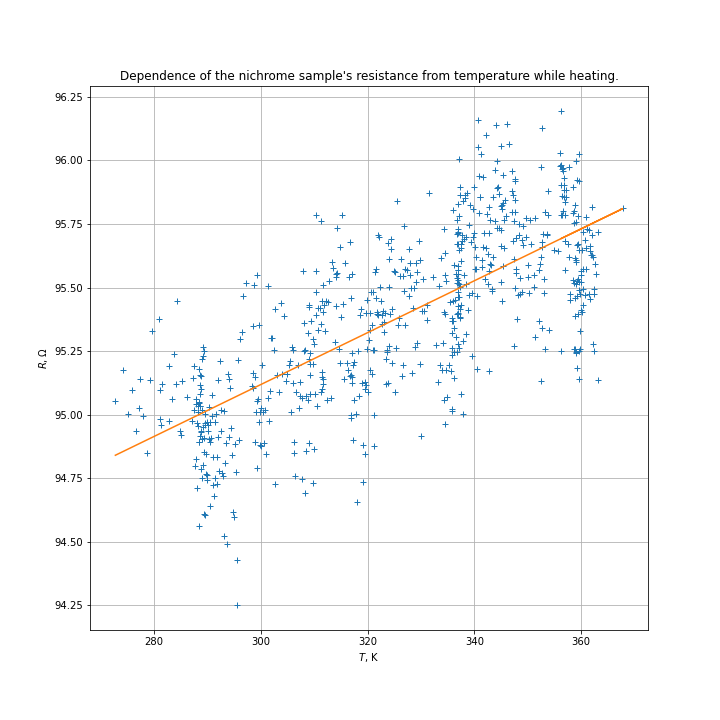
\includegraphics[width=\linewidth]{1_Ni_Heating}
	\caption{Зависимость сопротивления образца нихрома от температуры при нагреве с комнатной температуры до температуры, близкой к температуре кипения воды.}
	\label{fig:1_Ni_Heating}
\end{figure}

\subsection{Выводы}

\begin{enumerate}
	\item Получены навыки работы с жидким азотом, платиновым термометром.
	
	\item Полученные температурные коэффициенты электрического сопротивления (при температуре 298 К) при охлаждении ($\alpha_{\text{Cu}} = 0.00452 \text{ К}^{-1}$, $\alpha_{\text{Nic}} = 0.00017 \text{ К}^{-1}$) и при нагреве ($\alpha_{\text{Cu}} = 0.00397 \text{ К}^{-1}$, $\alpha_{\text{Nic}} = 0.00018 \text{ К}^{-1}$) с хорошей точностью совпадают с табличными ($0.004 \text{ К}^{-1}$ для меди и $0.0002 \text{ К}^{-1}$ для нихрома).
\end{enumerate}

\newpage

\section{Зависимость вида ВАХ диода от температуры}
\fancyhead[R]{\textsc{Зависимость вида ВАХ диода от температуры}}%Вставить колонтитул сюда

\subsection{Постановка целей работы}

Перед началом работы группой были поставлены следующие задачи:

\begin{enumerate}
	\item Собрать установку для определения вольт-амперной характеристики (ВАХ) диода и светодиода
	
	\item Получить зависимость формы ВАХ от температуры для диода
	
	\item Получить зависимость формы ВАХ от температуры для светодиода
\end{enumerate}

\subsection{Теоретическое введение}

\subsubsection{Описание энергетических диаграмм}

Опишем энергетические диаграммы pn-переходов различных состояниях, основываясь на \cite{Glazkov}.

Сразу же отметим знание, что при $T = 0$ уровень химического потенциала в чистом полупроводнике находится посередине запрещенной зоной, в то время как в легированных (имеющих избыток электронов/дырок) --- посередине между примесным уровнем и ближайшей зоной. При изменении температуры уровень химпотенциала будет смещаться и направление смещения будет зависеть от параметров самого полупроводника.

При первоначальном соединении полупроводников p-типа и n-типа произойдёт перераспределение зарядов до достижения нового положения равновесия. Условием термодинамического равновесия в присутствии электрического поля является постоянство по системе электрохимического потенциала, который для электронов равен $\mu - e \phi$ (знак минус связан с отрицательностью заряда электрона). Различие в положении уровня химпотенциала в соединяемых полупроводниках будет компенсироваться электростатическим потенциалом, возникающим при перераспределении зарядов.



На большом удалении от перехода концентрация зарядов равновесная и электростатический потенциал перераспределённых зарядов не зависит от координаты, в n-области уровень химпотенциала находится вблизи дна зоны проводимости, в p-области — вблизи потолка валентной зоны. При соединении полупроводников электрохимический потенциал, равный $\mu - e\phi = \text{const.}$ постоянен. В силу того, что $\mu_n > \mu_p$, электростатический потенциал $\phi$ в области n положителен относительно потенциала p-области. Электростатический потенциал должен быть непрерывным, а $\mu - e\phi = \text{const.}$, откуда делаем вывод, что $\mu$ также непрерывен, т.е. в окрестности перехода уровень химпотенциала должен плавно измениться от положения вблизи дна зоны проводимости в n-области к положению вблизи потолка валентной зоны в p-области (см. рисунок \ref{fig:2_zones_not_cool}).

\begin{figure}[H]
	\centering
	\includegraphics[width=0.7\linewidth]{2_zones_not_cool}
	\caption{Энергетическая диаграмма p-n перехода для случая контакта полупроводника одного типа с различным легированием. Слева n-область, справа p-область. Уровни химпотенциала соединены схематически.}
	\label{fig:2_zones_not_cool}
\end{figure}

Эту картину можно перестроить. Для этого построим энергетическую диаграмму для полной энергии, ,,добавив'' потенциальную энергию к уже отражённой в нашем рисунке зонной структуре (потенциальная энергия электрона в электрическом поле есть $U = -e\phi$). Тогда в силу уже обговоренного $\mu - e\phi = \text{const.}$ это построение приобретёт простой графический смысл: уровень химпотениала станет постоянен по рисунку (теперь это электрохимпотенциал), а так как ширина запрещённой зоны и расстояние от уровня химпотенциала до потолка или дна зоны или до примесного уровня при этом перестроении не меняются, то возникает так называемый изгиб зон (см. рисунок \ref{fig:2_zones_cool}).

\begin{figure}[H]
	\centering
	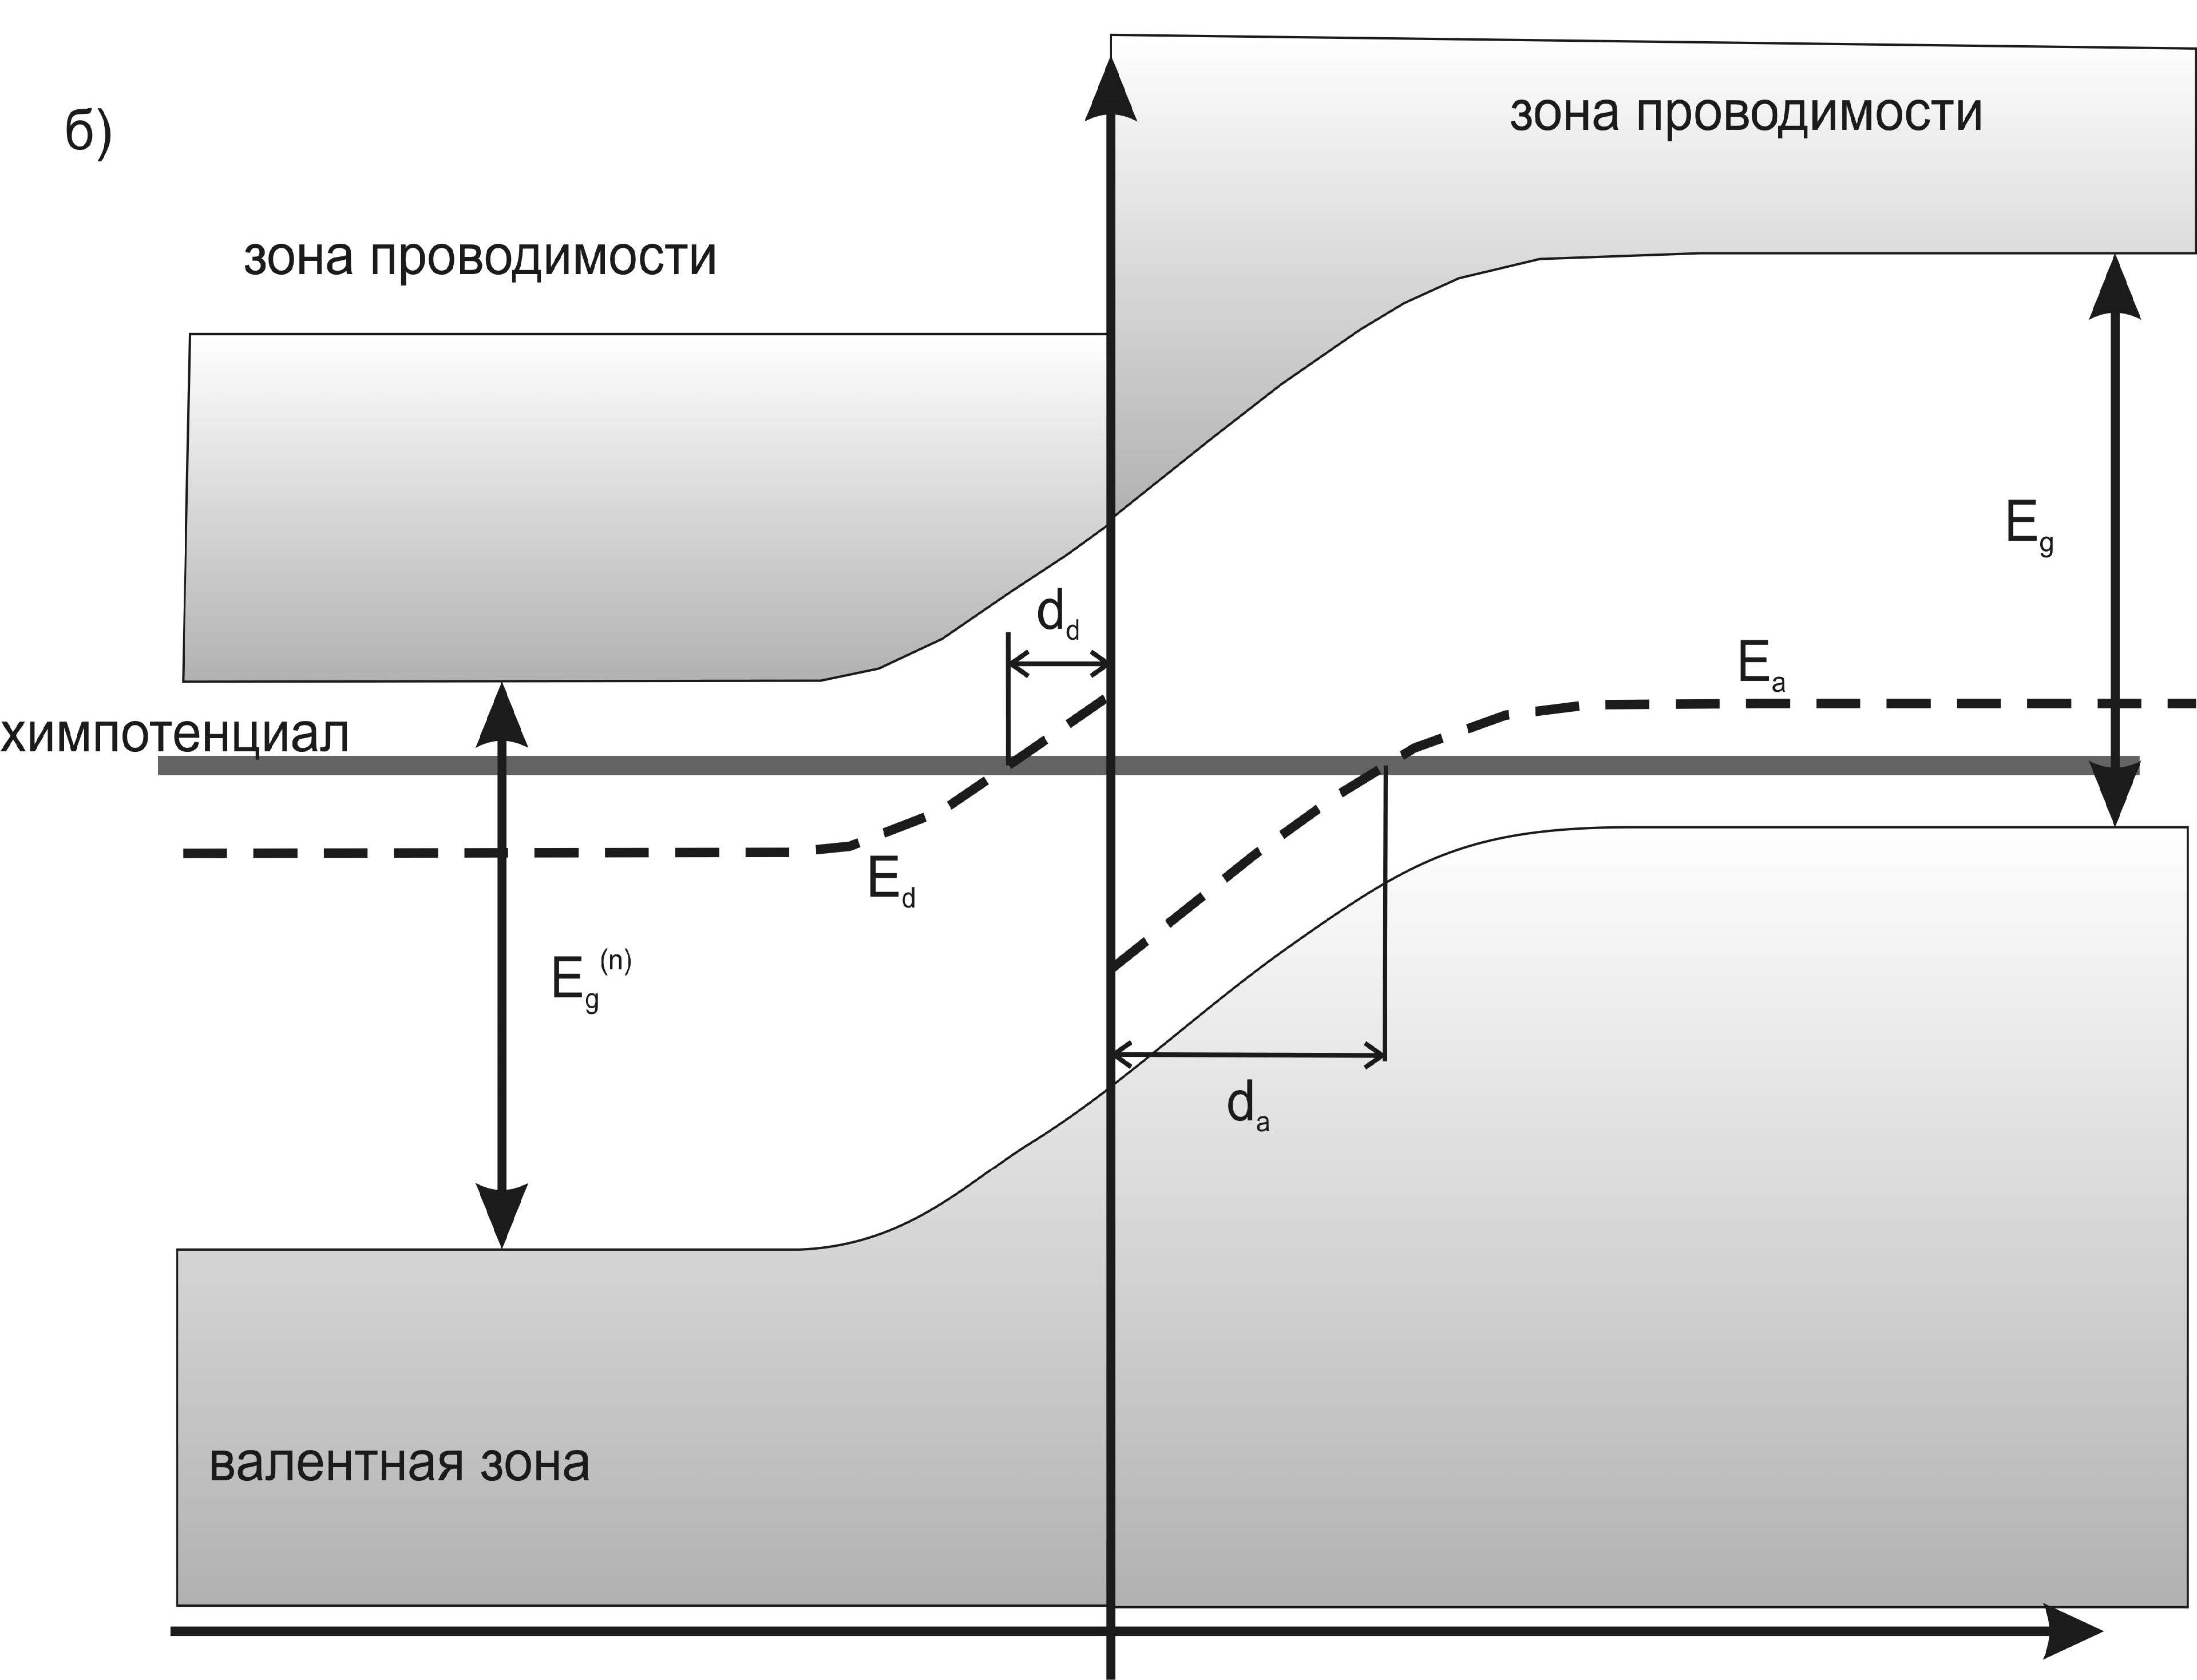
\includegraphics[width=0.7\linewidth]{2_zones_cool}
	\caption{Энергетическая диаграмма p-n перехода для случая контакта полупроводника одного типа с различным легированием. Слева n-область, справа p-область. Изгиб зон при представлении энергетической диаграммы для полной энергии.}
	\label{fig:2_zones_cool}
\end{figure}

Закончив эту необходимую вводную, перейдем, наконец, к описанию энергетических диаграмм в различных состояниях pn-перехода.

Сразу отметим, что в присутствии источника напряжения ситуация резко становится неравновесной: источник всё время совершает работу для поддержания заданной разности потенциалов и по переходу течёт ток. Приложение напряжения к переходу приводит к двум эффектам: возникает ток носителей, поддерживаемый источником, и изменяется картина перераспределения зарядов на границе. Эти явления можно разделить при рассмотрении: перераспределение зарядов создаёт некоторый рельеф потенциала внутри образца, а ток носителей происходит по этому рельефу, под действием вынуждающей силы внешнего источника.

Если мы приложим к переходу некоторое напряжение $V_{\text{ext}}$, то теперь при переносе электронов между приводимыми в контакт областями нужно учесть, что дно зоны проводимости в p-области дополнительно сместилось относительно уровня минимальной энергии электрона в вакууме на $-eV_{\text{ext}}$. Из-за этого, разумеется, смещается и положением химпотенциала, примесного уровня и потолка валентной зоны.

С точки зрения энергетической диаграммы для полной энергии (а на ней уровень химпотенциала в отсутствии напряжения был постоянным) это значит, что для того, чтобы показать новый установившийся рельеф, нам нужно сместить уровень химпотенциала вдали от перехода в p-области на $-eV_{\text{ext}}$ и достроить зависимость химпотенциала до непрерывности в переходной области.

Рассмотрим теперь концентрации. В отсутствие внешнего напряжения концентрация электронов на одном уровне нашей энергетической диаграммы одинакова в обоих полупроводниках: она определяется только расстоянием до этого уровня от спрямлённого в этом представлении уровня химпотенциала. Аналогичное верно и для дырок. Естественно, что в таком случае ток не течет (нет перепада концентрации и токи слева направо и справа налево компенсируют друг друга). При приложении внешнего напряжения уровень химпотенциала сдвигается. Для определенности в описании предположим, чтобы было приложено напряжение $V_{\text{ext}} > 0$. На том же уровне энергии при этом в p-части оказывается меньше электронов, чем в n-части, из-за чего возникает электронный ток слева направо (в нашем случает) и дырочный ток в обратном направлении.

Конкретизируем размышления: пусть $V_{\text{ext}} > 0$ мало. В таком случае могут переходить только те электроны, чья энергия выше уровня дна зоны проводимости в полупроводнике p-типа, и дырки, энергия которых на диаграмме ниже уровня потолка валентной зоны в полупроводнике n-типа. При относительно небольшой температуре таких электронов не так много вследствие их распределения по энергиям, поэтому при небольших напряжениях ток через переход мал (см. рисунок \ref{fig:2_schemes} здесь и в дальнейших описаниях энергетических диаграмм).

\begin{figure}[H]
	\centering
	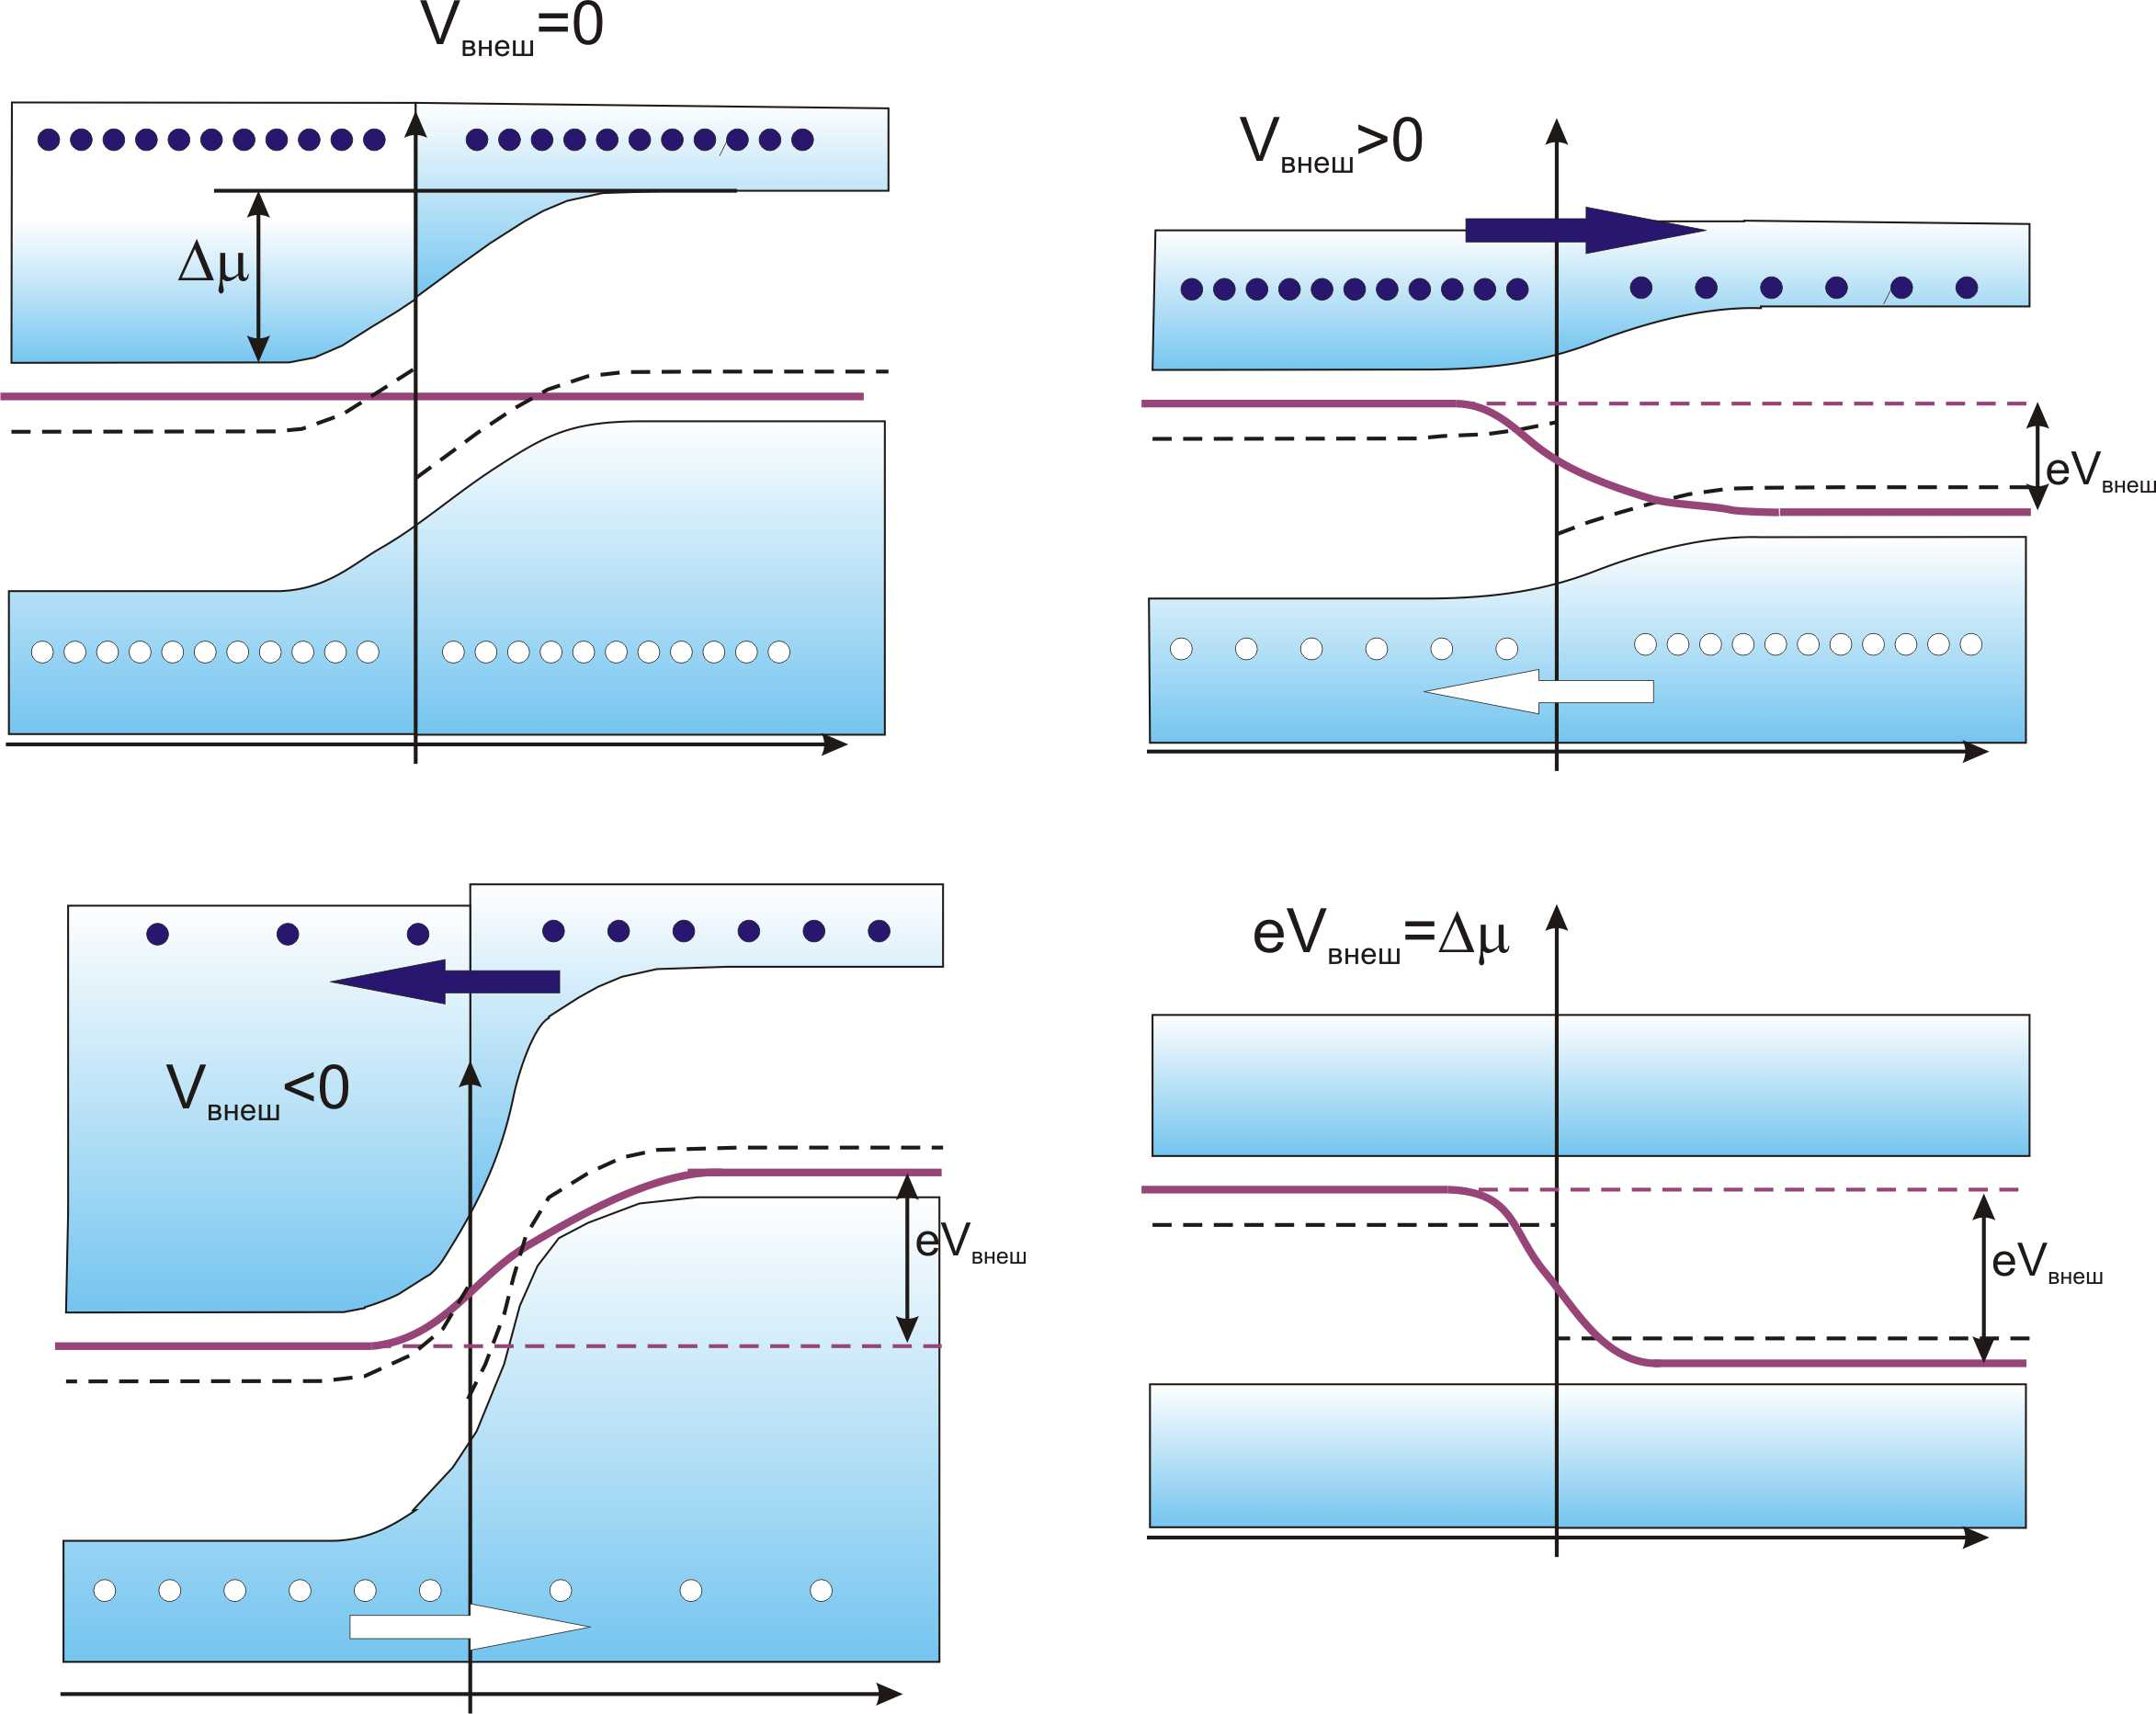
\includegraphics[width=\linewidth]{2_schemes}
	\caption{Построение схемы энергетической диаграммы для p-n перехода с приложенным внешним напряжением. Слева полупроводник n-типа, справа --- p-типа.}
	\label{fig:2_schemes}
\end{figure}

Подобный режим сохраняется вплоть до момента $e V_{\text{ext}} = \Delta \mu$, в который происходит открытие диода. С этого момента \textbf{все} основные носители могут проходить через переход и ток экспоненциально возрастает.

Скажем также буквально пару слов про ситуацию $e V_{\text{ext}} < 0$, т.е. при обратной полярности. В этом случае переход для основных носителей всегда заперт. При такой полярности, однако, могут проходить неосновные носители заряда, который дают небольшой ток.

% Наконец, заметим, что выпрямляющее действие p-n перехода оказывается однозначным следствием изгиба зон. Изгиб зон возникает вследствие различия положения химпотенциала в соединяемых полупроводниках. Следовательно, при повышении температуры, когда становится главным вклад собственных носителей заряда и химпотенциал смещается к центру запрещённой зоны, выпрямляющее действие p-n перехода пропадёт.

\subsubsection{Вывод формулы ВАХ}

Чтобы вывести формулу вида ВАХ обратимся к \cite{Igoshin}. Сперва подсчитаем разность потенциалов, возникающую у полупроводника в области pn-перехода. Для этого учтем, что при равной концентрации акцепторов и доноров (а это верно в случае статической ситуации) смещение уровня Ферми вверх в n-области равно смещению его же в p-области, поэтому для разности потенциалов $\Delta V$ можно записать: 

\begin{equation}
	e\Delta V = 2 \left(\mu - \frac{1}{2} E_{\text{c}}\right)
\end{equation}

В этой формуле энергия уровней отсчитывается от верхнего края валентной зоны, а величина $E_{\text{c}}/2$ определяет несмещенное положение уровня Ферми.

Плотность электронов в зоне проводимости при обычных температурах определяется только теми электронами, которые даются донорными уровнями. Она равна:

\begin{equation}
	n_n = Q_n \exp\left(-\frac{E_{\text{c}} - \mu}{k_B T}\right)
\end{equation}

Плотность дырок же в валентной зоне равна плотности электронов, перешедших под действием теплового возбуждения из валентной зоны в зону проводимости, т.е.:

\begin{equation}
	n_p = Q_p \exp\left(-\frac{\mu}{k_B T}\right)
\end{equation}

Поделим два последних равенства друг на друга с учетом того, что $Q_n = Q_p$ и получим выражение для искомой разности потенциалов через концентрации:

\begin{equation}
	\frac{n_n}{n_p} = \exp\left(\frac{2\mu - E_\text{c}}{k_B T}\right) = \exp\left(\frac{e \Delta V}{k_B T}\right) \qrq \Delta V = \frac{k_B T}{e} \ln \frac{n_n}{n_p}
\end{equation}

Как уже было сказано, из-за наличия потенциального барьера между концентрациями основных и неосновных носителей заряда в n- и p- Областях устанавливается определенное соотношение. Для равновесия запишем:

\begin{equation}
	\frac{n_n(\text{n-область})}{n_n(\text{p-область})} = \frac{n_p(\text{p-область})}{n_p(\text{n-область})} = \exp\left(\frac{e \Delta V}{k_B T}\right)
\end{equation}

Интерпретируем полученное соотношение: в материале n-типа имеется высокая концентрация электронов. Однако лишь небольшая их часть $\exp\left[-e\Delta V / (k_B T)\right]$, поднимаясь как бы ,,в горку'' проходит в материал p-типа. Этими электронами образуется поток, который проходит через переход с одной стороны. С другой стороны имеется такой же в случае равновесия ток. Указанный ток не уменьшается из-за контактной разности потенциалов, т.к. в этом случае электроны с горки ,,скатываются''. Обозначим величину этих токов как $I_0$, тогда:

\begin{equation}
	I_0 \sim n_n(\text{p-область}) = n_n(\text{n-область})\exp\left(-\frac{e\Delta V}{k_B T}\right)
	\label{eq:2_I}
\end{equation}

Теперь приложим к переходу некоторое напряжение $V_\text{ext}$ от внешнего источника так, чтобы p-область заряжалась положительно относительно n-области. Проводимость перехода крайне мала, из-за чего это напряжение практически полностью на нем падает. Потенциальная энергия электронов в p-области снижается по сравнению с n-областью на логичную величину $eV_{\text{ext}}$, соответственно, понижается и положение уровня Ферми.

Ток, проходящий справа налево в такой ситуации не меняется и по-прежнему равен $I_0$. Ток же, проходящий справа налево --- из-за снижения барьера --- соответственно возрастает в $\exp[eV_{\text{ext}} / (k_B T)]$. Полный же ток равен разности этих двух токов, т.е.:

\begin{equation}
	I(V_\text{ext}) = I_0 \left[\exp\left(\frac{e V_{\text{ext}}}{k_B T}\right) - 1\right]
	\label{eq:2_I(V)}
\end{equation}

Все вышесказанное применимо и к току, переносимому дырками. Полученная формула корректно описывает и полный ток, проходящий через переход, если понимать под $I_0$ ток, переносимый в равновесии как электронами, так и дырками.

Чтобы, однако, получить итоговую формулу для ВАХ перехода, сделаем последний штрих: подставим \ref{eq:2_I} в полученную \ref{eq:2_I(V)} (учтя при этом упомянутую ремарку, что измеряемый на опыте ток равен сумме тока электронов и тока дырок):

\begin{align*}
	I(V_{\text{ext}}) = (I_{0, n} + I_{0, p}) \left[\exp\left(\frac{e V_{\text{ext}}}{k_B T}\right) - 1\right] = \\ = [n_n(\text{n-область}) + n_p(\text{p-область})]\exp\left(-\frac{e \Delta V}{k_B T}\right) \left[\exp\left(\frac{e V_{\text{ext}}}{k_B T}\right)\right]
\end{align*}

В формуле учтено сказанное выше про то, что $n_n$ и $n_p$ определяются концентрацией акцепторных и донорных примесей и слабо зависят от температуры. По этой причине они были заменены константами. ВАХ, получаемая по такой формуле, изображена на рисунке \ref{fig:2_VAC}.

\begin{figure}[H]
	\centering
	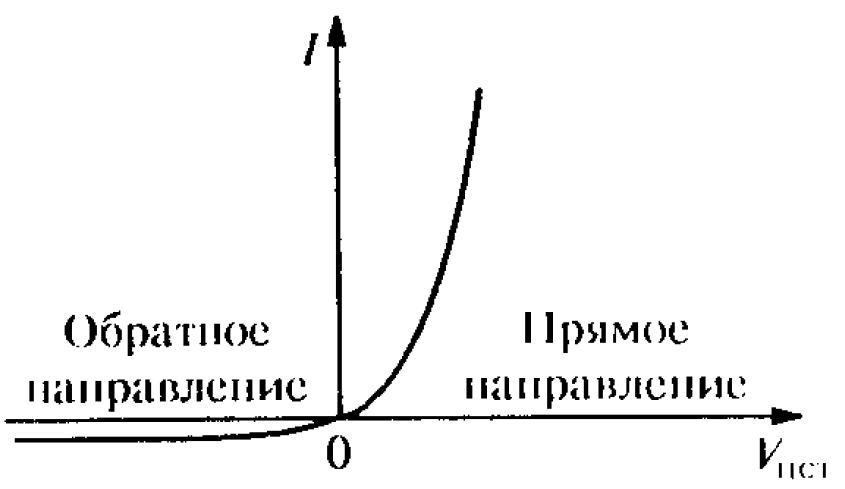
\includegraphics[width=0.5\linewidth]{2_VAC}
	\caption{Зависимость силы тока, проходящего через pn-переход, от напряжения, приложенного к переходу.}
	\label{fig:2_VAC}
\end{figure}

\subsection{Описание установки}

Для проведение эксперимента была предложена схема с использованием осциллографа, который одновременно выступает в роли генератора синусоидального сигнала, представленная на рисунке \ref{fig:2_Experiment_Scheme}.

\begin{figure}[H]
	\centering
	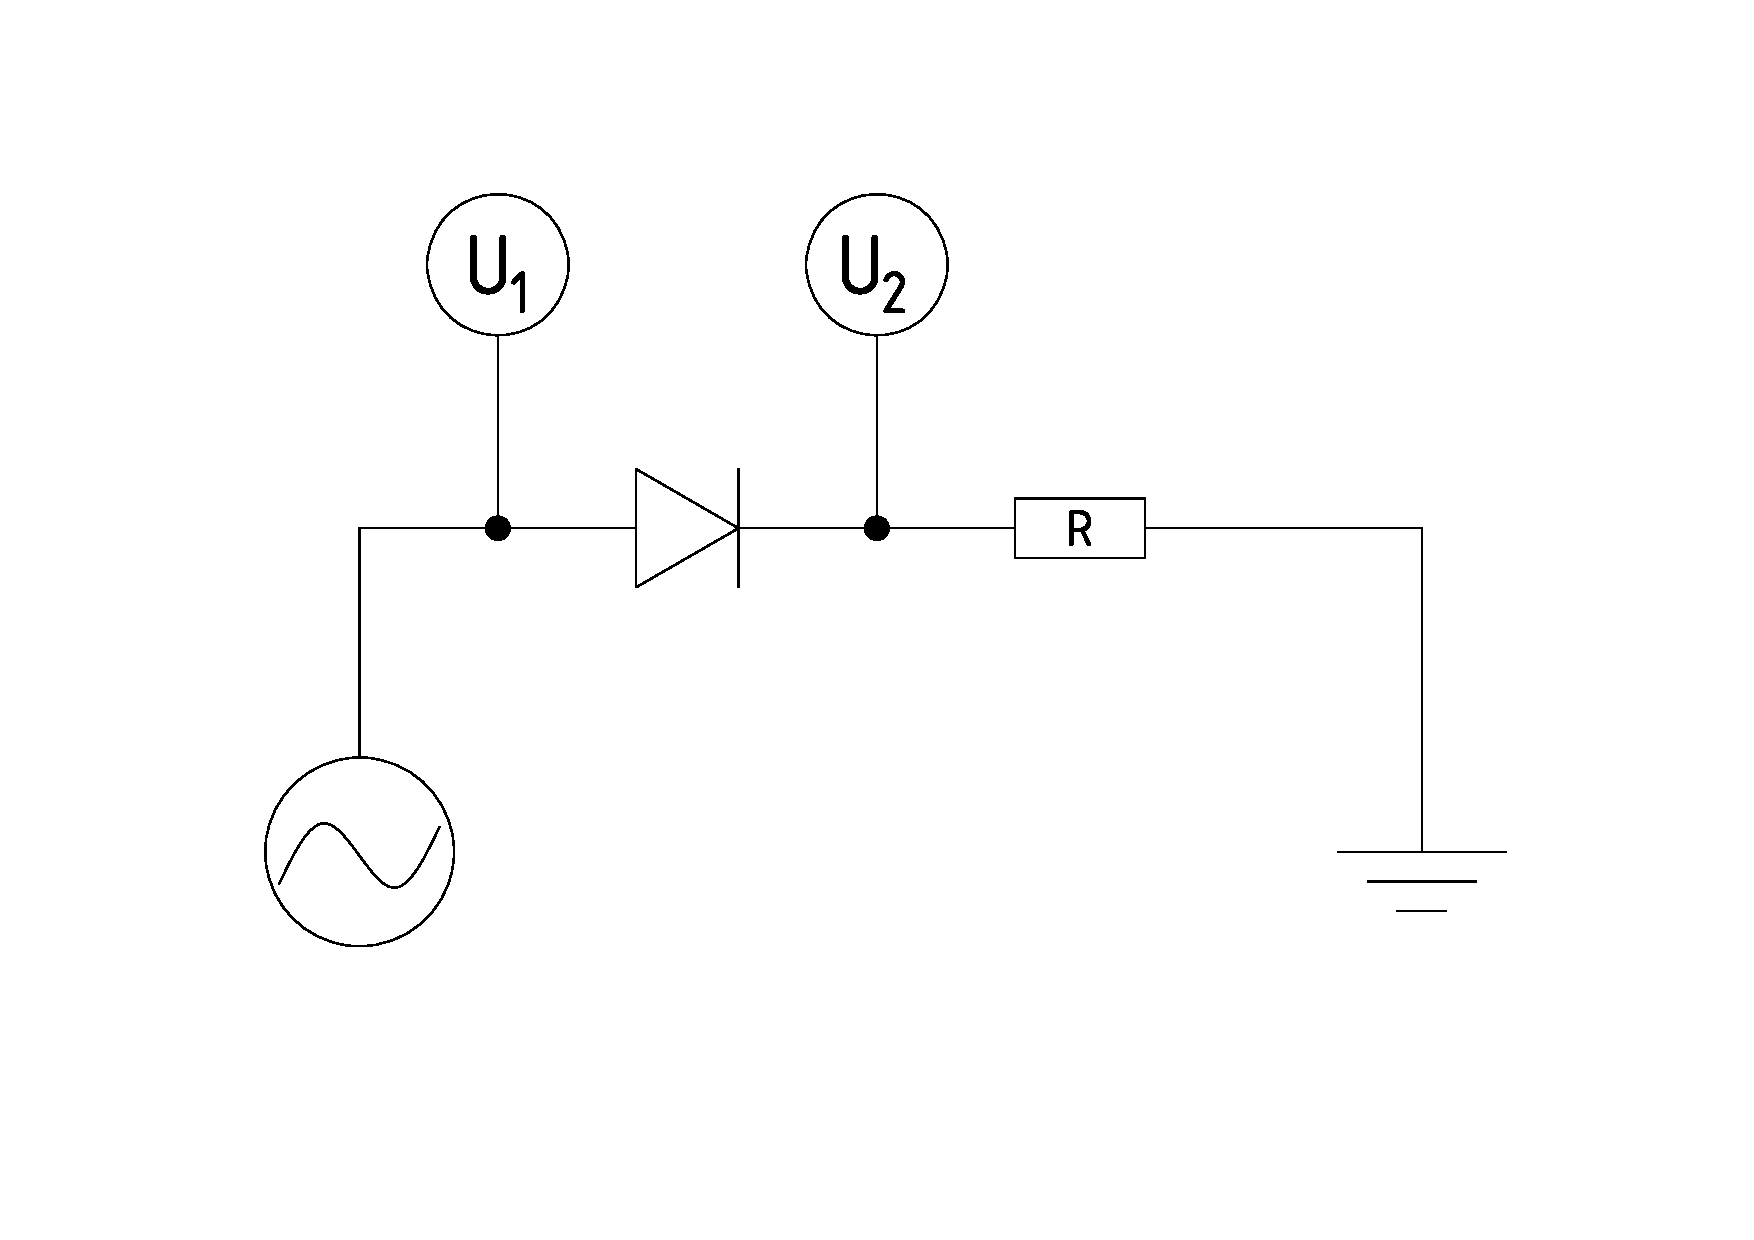
\includegraphics[width=\linewidth]{2_Experiment_Scheme}
	\caption{Электрическая схема для проведения эксперимента по получению ВАХ диодов.}
	\label{fig:2_Experiment_Scheme}
\end{figure}

\subsection{Анализ полученных результатов}

\subsubsection{Диод}

Полученные в ходе измерений данные визуализированы на рисунке \ref{fig:2_Diode}.

\begin{figure}[H]
	\centering
	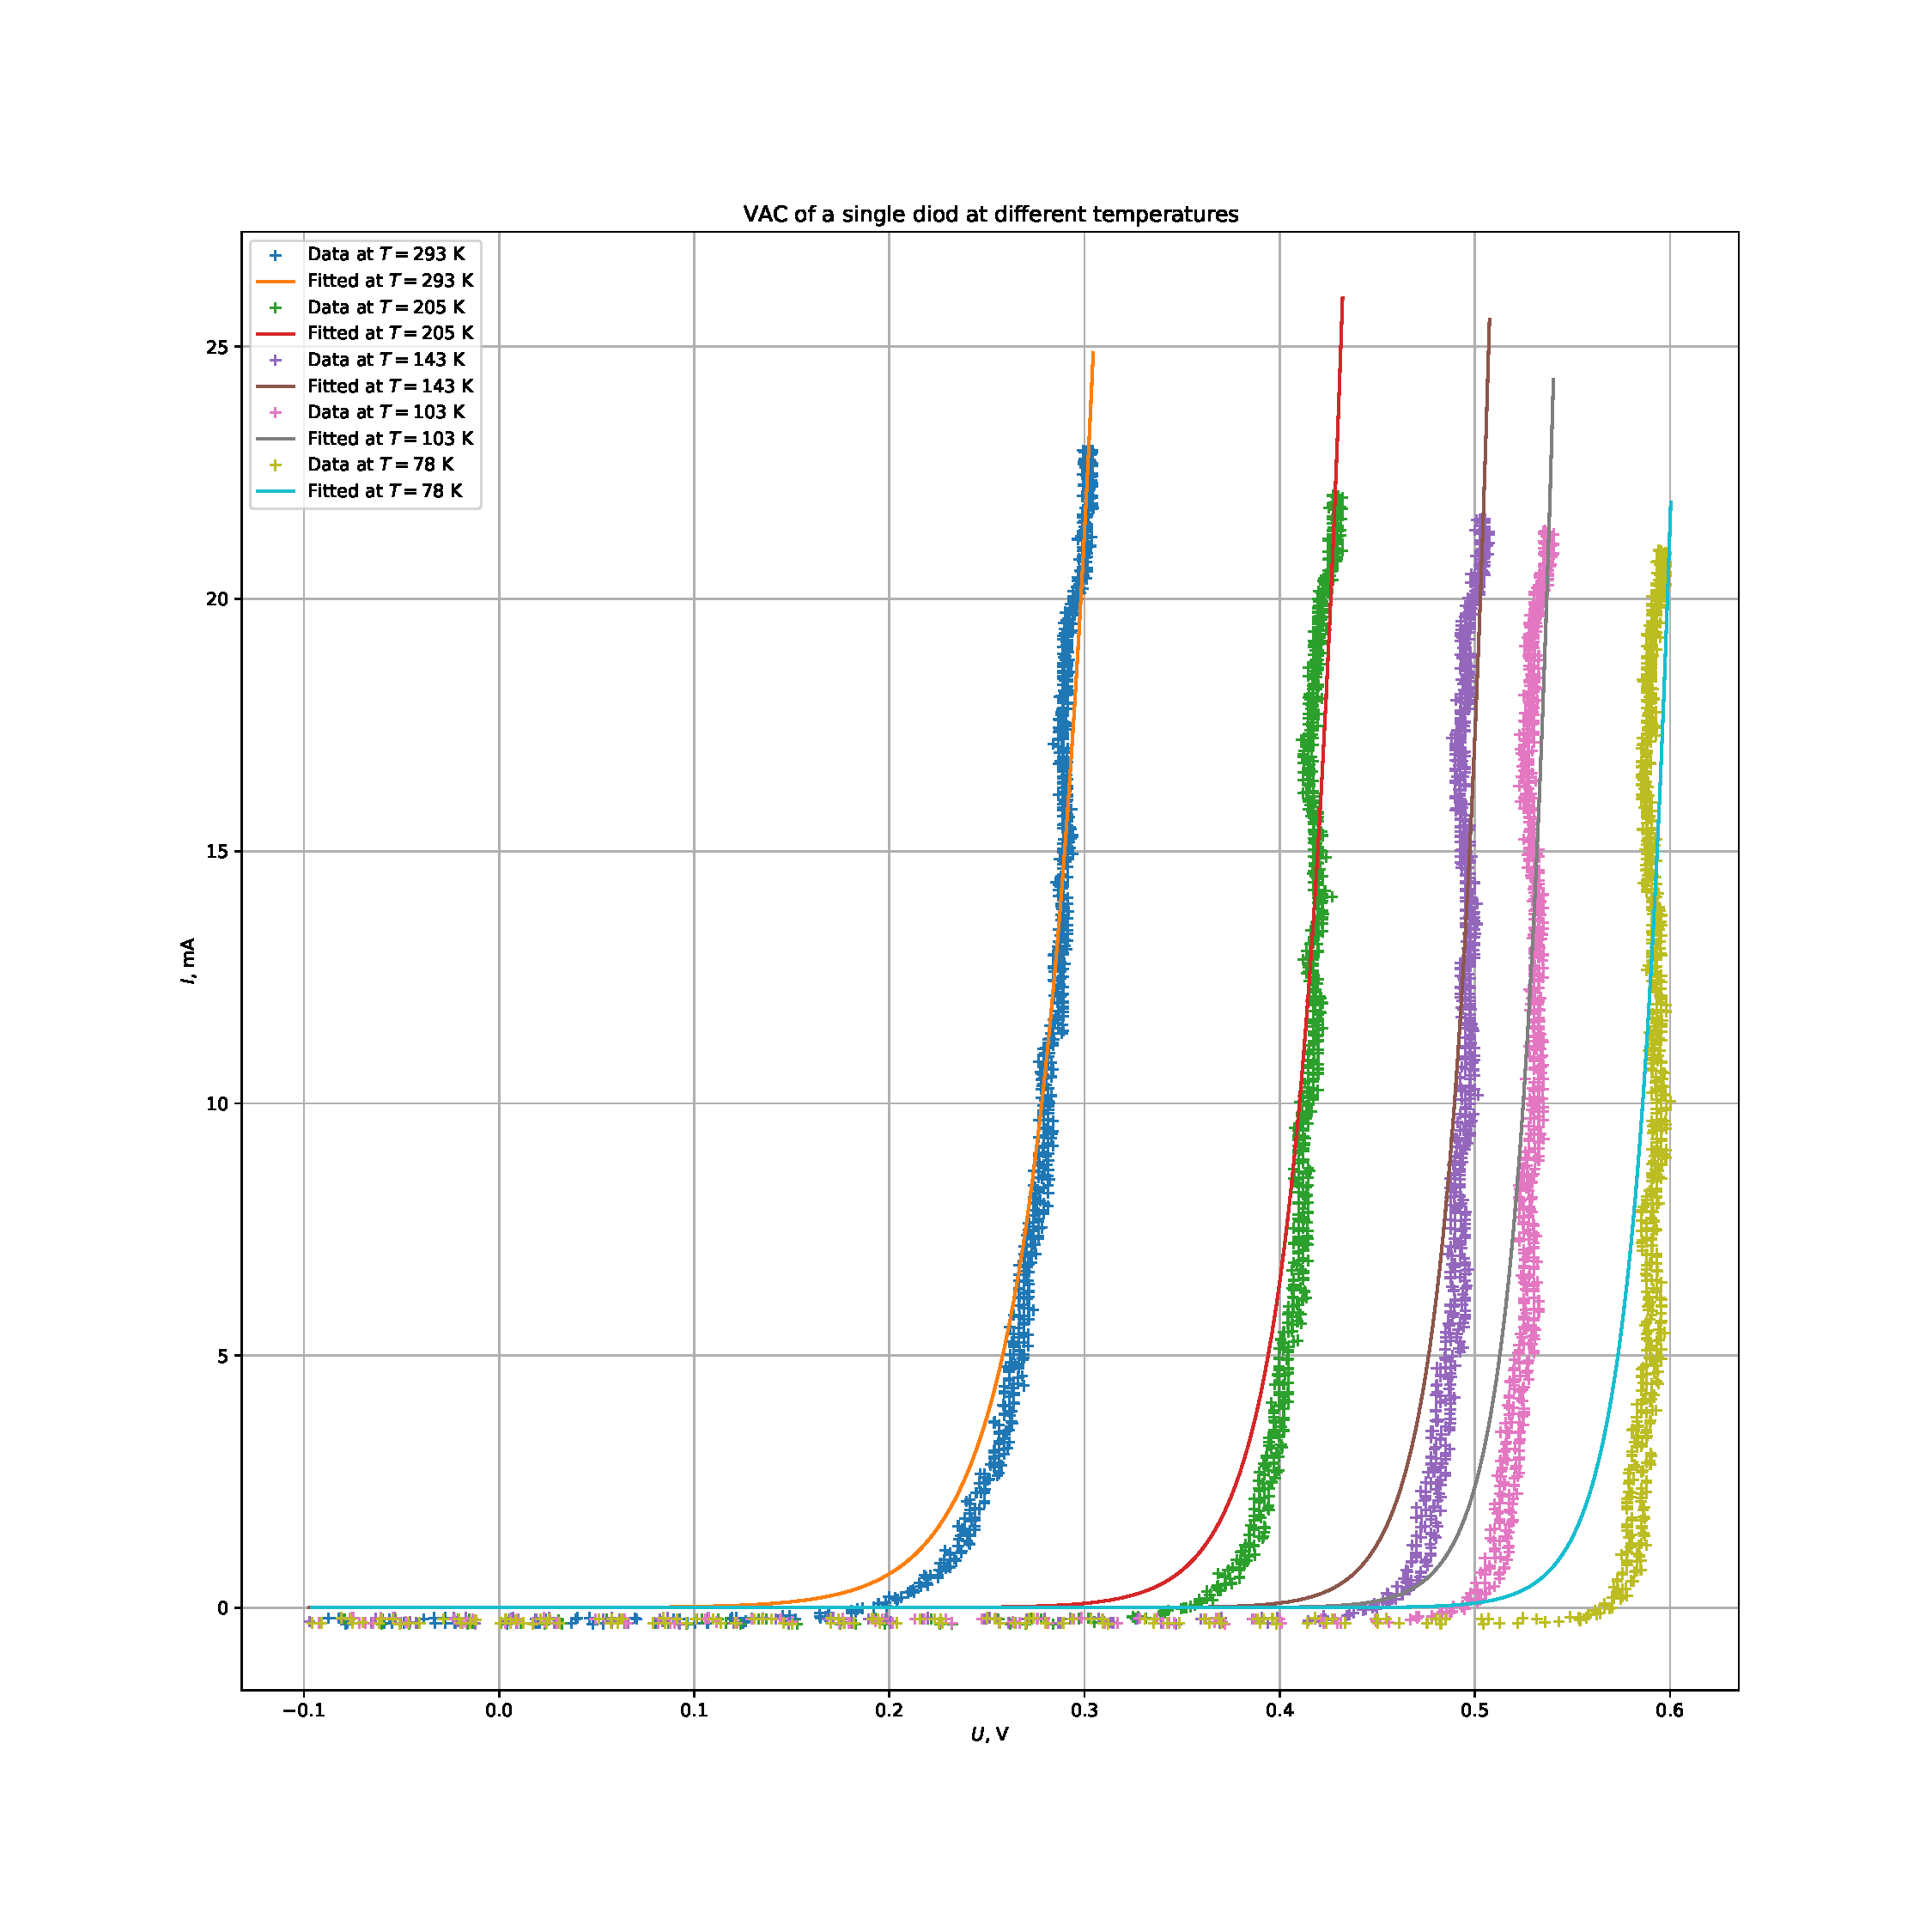
\includegraphics[width=\linewidth]{2_Diode}
	\caption{ВАХ-и диода при его различных температурах.}
	\label{fig:2_Diode}
\end{figure}

Из полученных графиков можно, например, вытащить зависимость напряжения, при котором открывается диод, от температуры. Полученная зависимость представлена на рисунке \ref{fig:2_Knee_Diode}. Основываясь на формуле \ref{eq:2_I} мы могли бы предполагать линейный рост напряжения с ростом температуры, однако происходит обратное: реально наблюдается линейное падение напряжения с ростом температуры. Это можно объяснить наличием у $I_0$ температурной зависимости вида:

\begin{equation}
	I_0 \sim \frac{1}{\exp[e b/(k_B T)] - c}
\end{equation}

Где $b, c$ --- постоянные, определяемые характером зависимости $V_{\text{ext}}$ от $T$.

\begin{figure}[H]
	\centering
	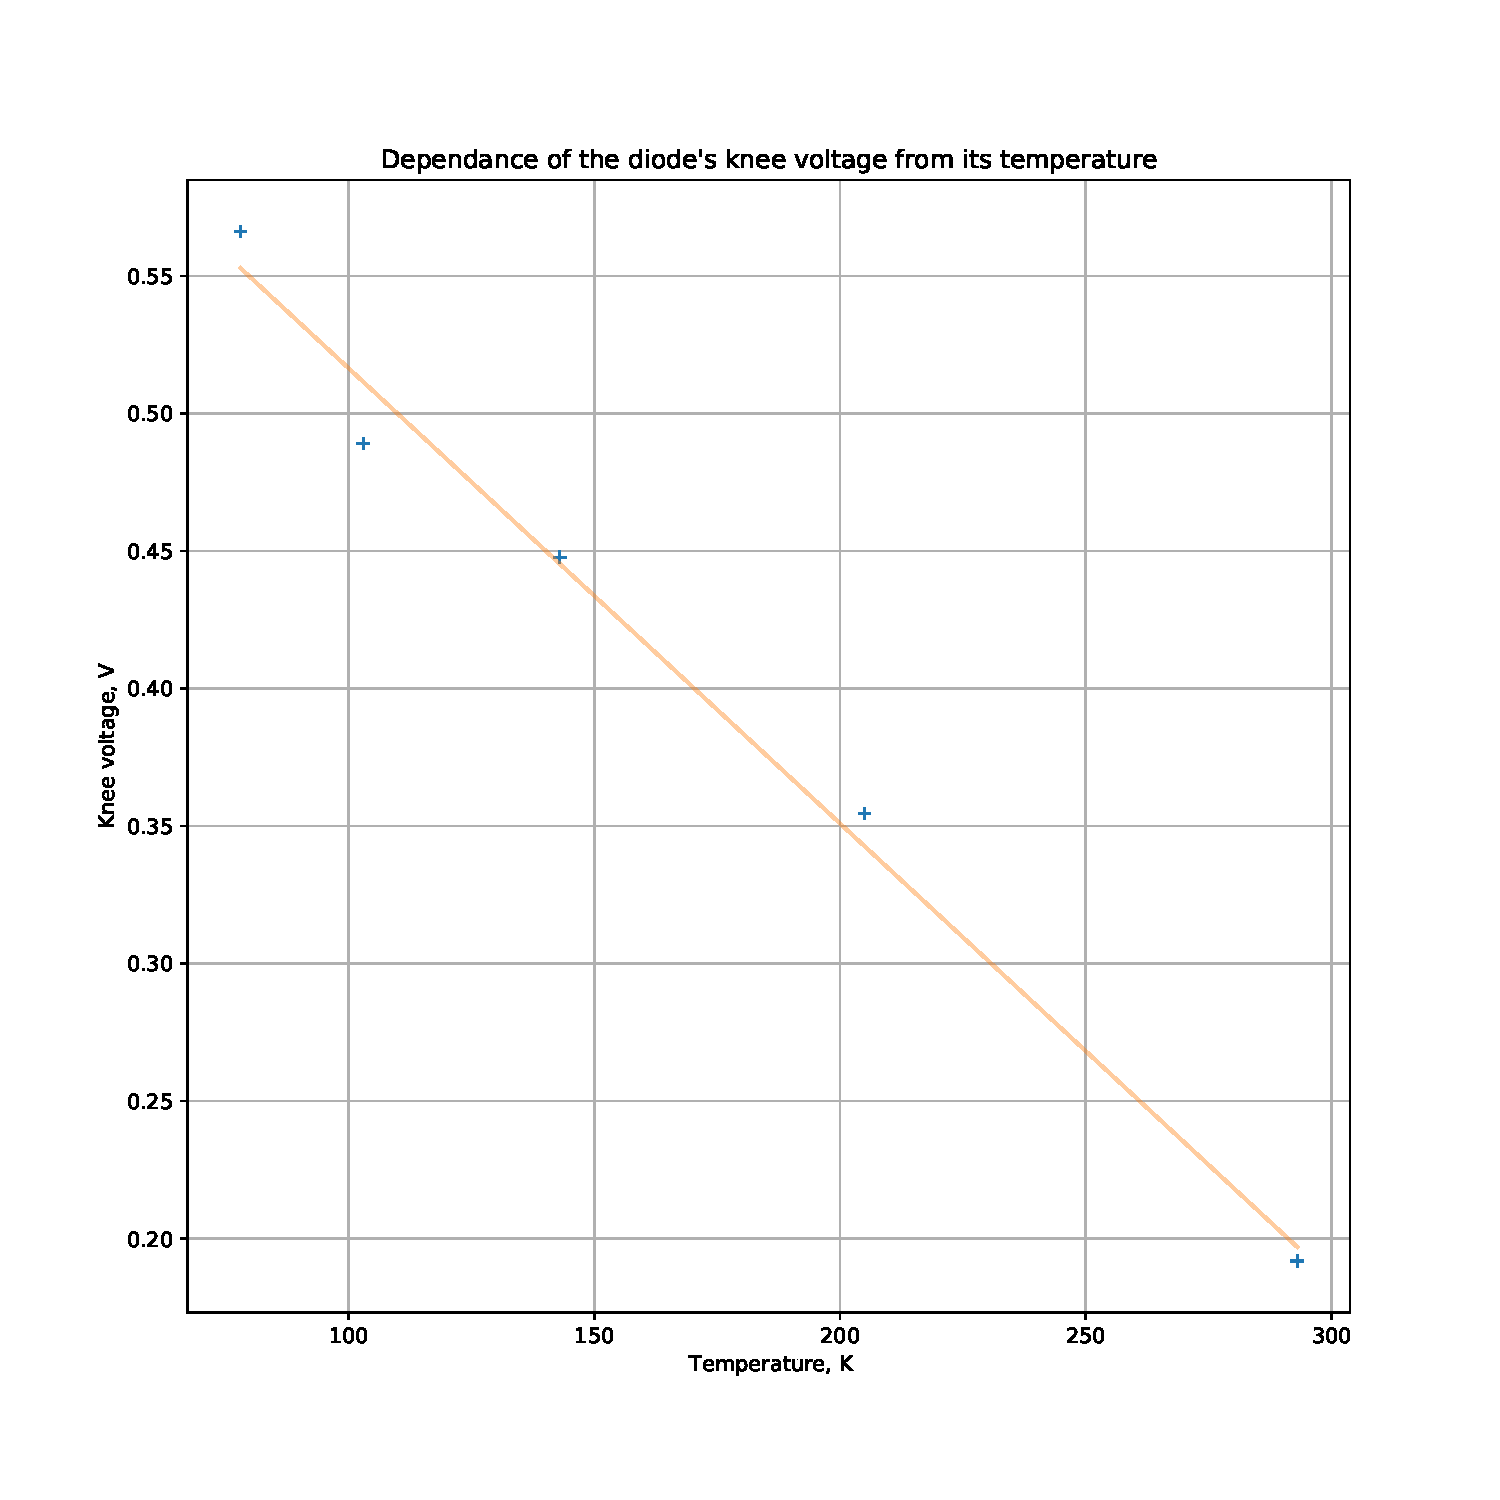
\includegraphics[width=\linewidth]{2_Knee_Diode}
	\caption{Зависимость напряжения, при котором происходит открытие диода, от его температуры.}
	\label{fig:2_Knee_Diode}
\end{figure}

Понятно, что такое поведение как минимум не до конца коррелирует с предсказанием, сделанным на основании теоретических выкладок. Однако необходимо понимать, что вывод формулы был произведен для случая идеального (а не реального) pn-перехода, и что в диоде потенциально может применяться не один pn-переход, а некоторая их композиция.

\subsubsection{Светодиод}

Как и раньше, представим собранные данные на рисунке \ref{fig:2_LED}.

\begin{figure}[H]
	\centering
	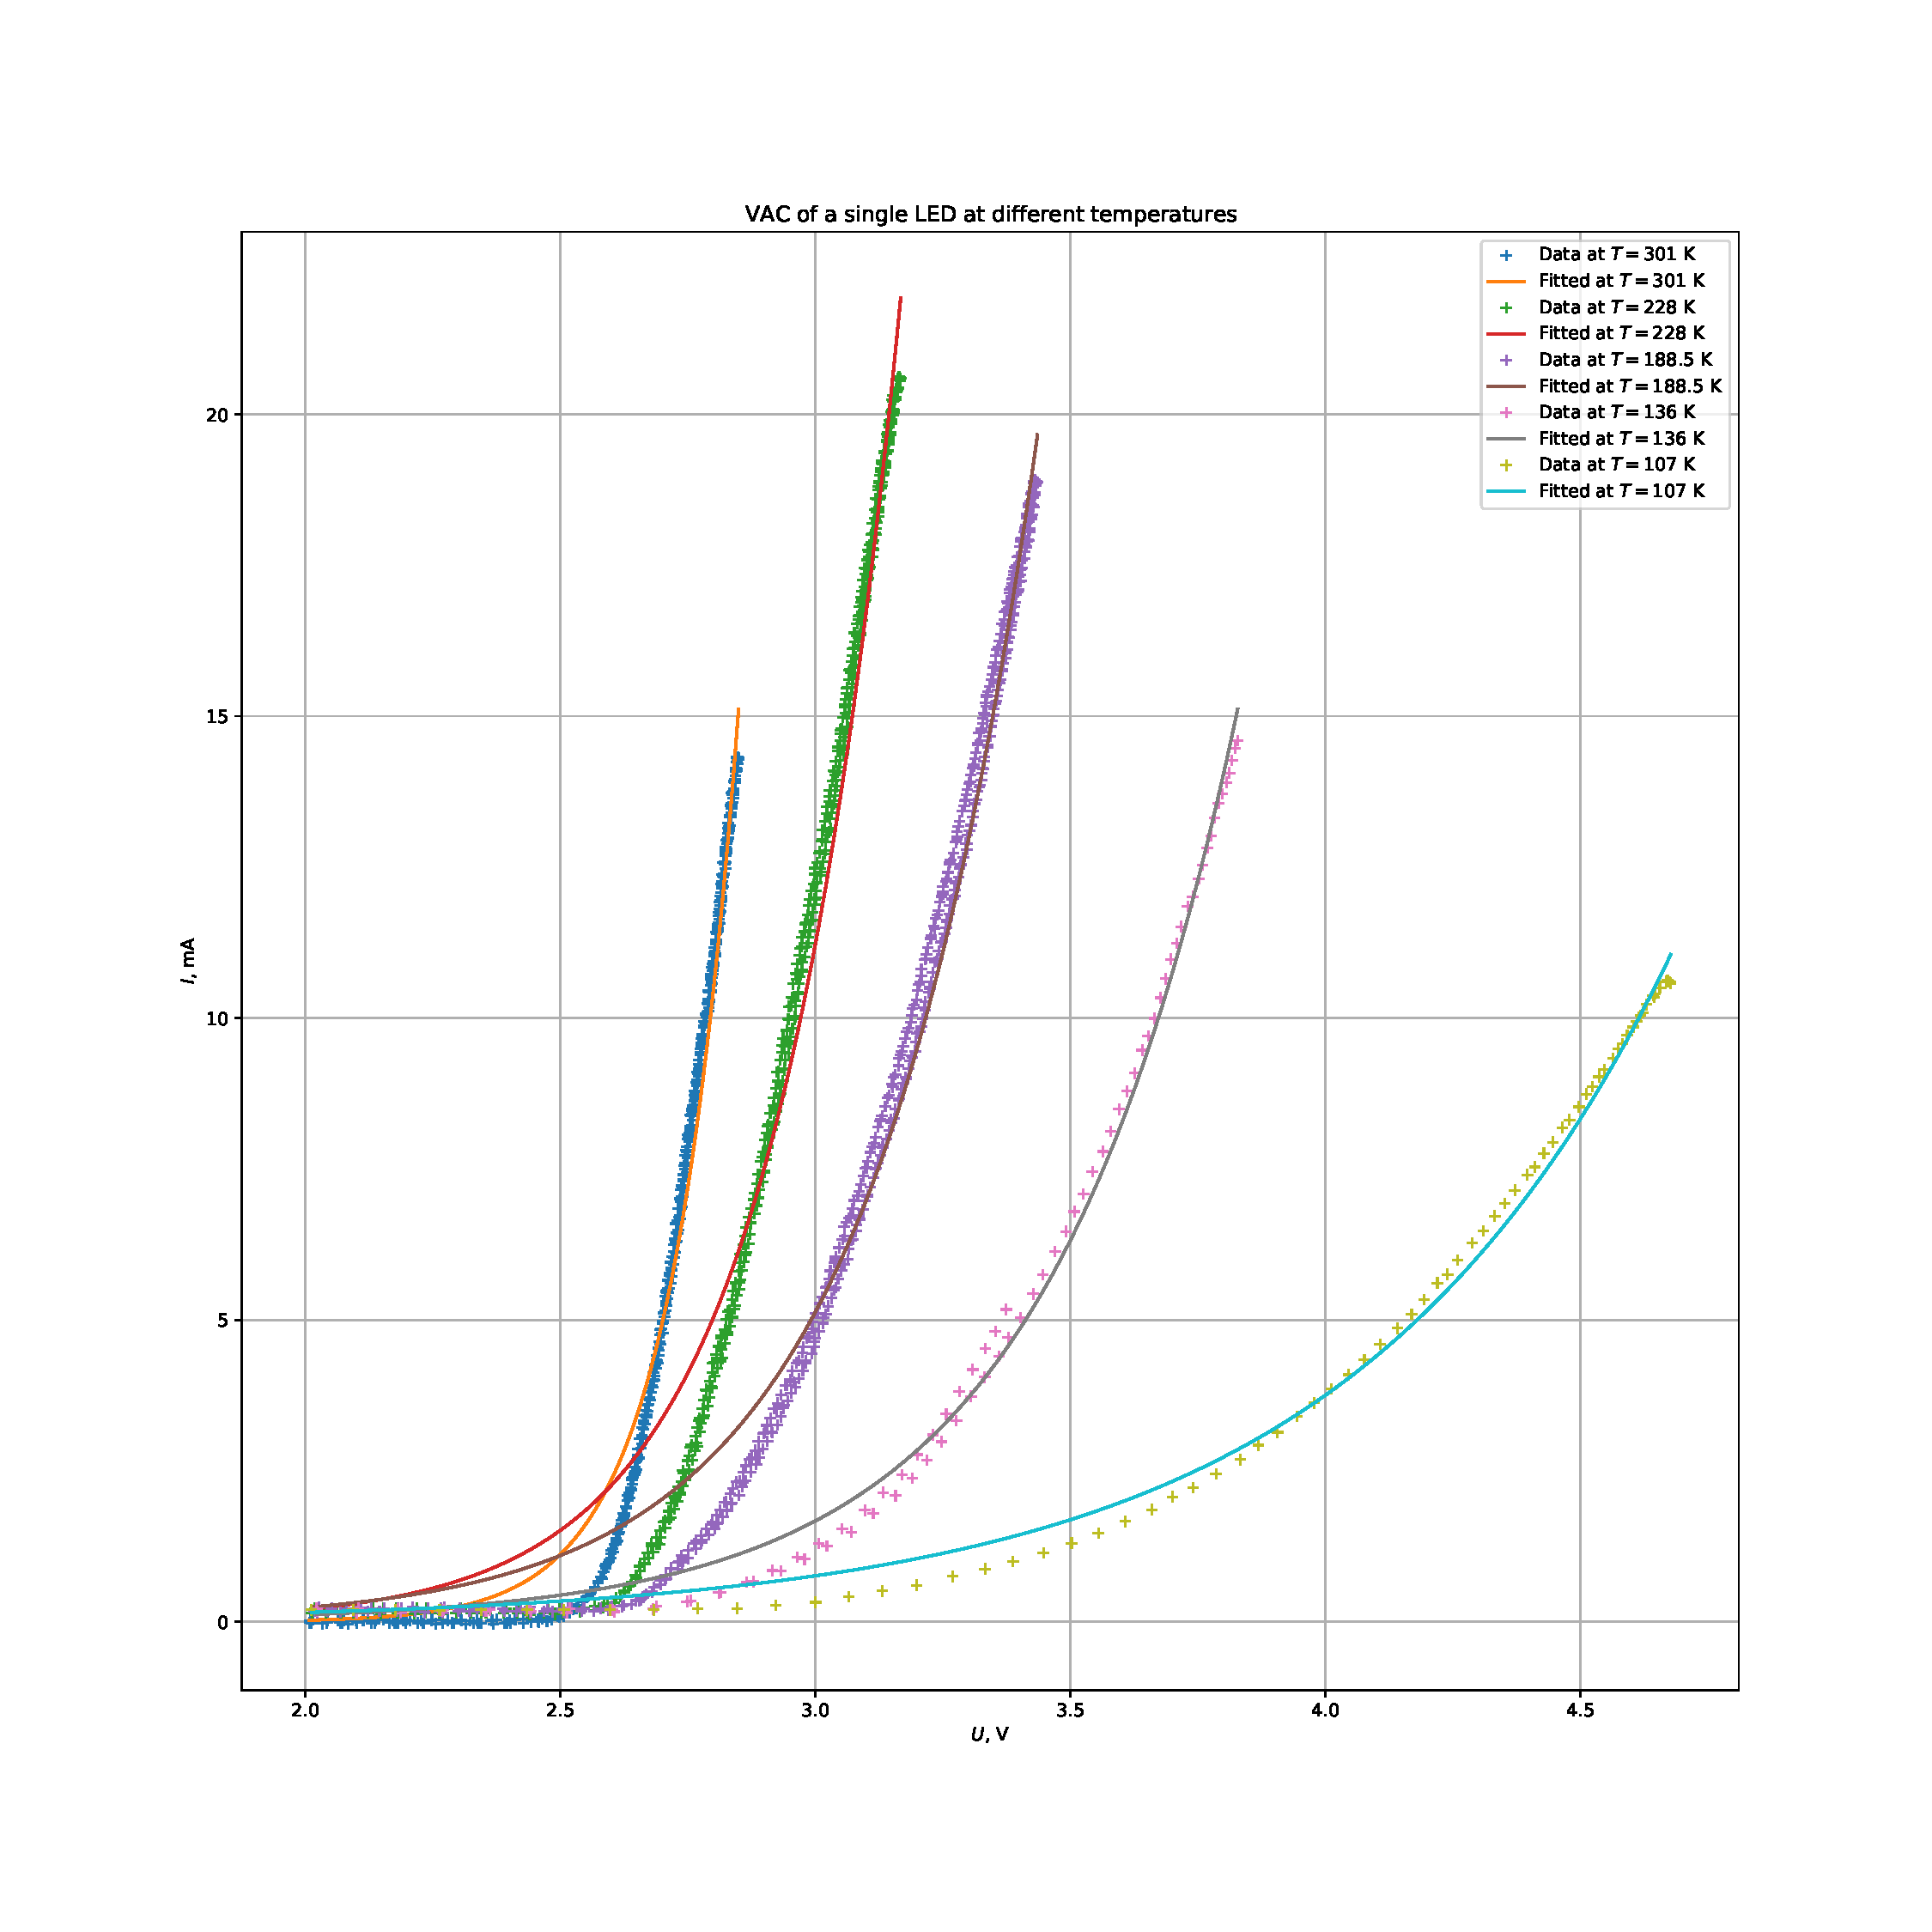
\includegraphics[width=\linewidth]{2_LED}
	\caption{ВАХ-и светодиода при его различных температурах.}
	\label{fig:2_LED}
\end{figure}

Из полученных графиков видно, что с уменьшением температуры ВАХ все больше похожа на экспоненту, в то время как ВАХ при более высоких температурах больше походят по внешнему виду на ВАХ обычного диода.

Как и прежде, попытаемся определить зависимость напряжения, при котором достигается некоторый небольшой ток, от температуры (назовем это аналогом напряжения открытия). Для этого обратимся к рисунку \ref{fig:2_Knee_LED}. Видно, что зависимость по своей форме напоминает $V\sim 1 / T$. Для достижения такой зависимости должно, предположительно, выполняться следующее:

\begin{equation}
	I_0 \sim \frac{1}{\exp[e a / (k_B T^2)] \cdot \exp[e b / (k_B T)] - 1}
\end{equation}

Как и прежде, $b, c$ --- постоянные, определяемые характером зависимости $V_{\text{ext}}$ от $T$.

Объяснение подобной зависимости $I_0$ от температуры $T$ предлагается такое же, как и при рассмотрении диода.

\begin{figure}[H]
	\centering
	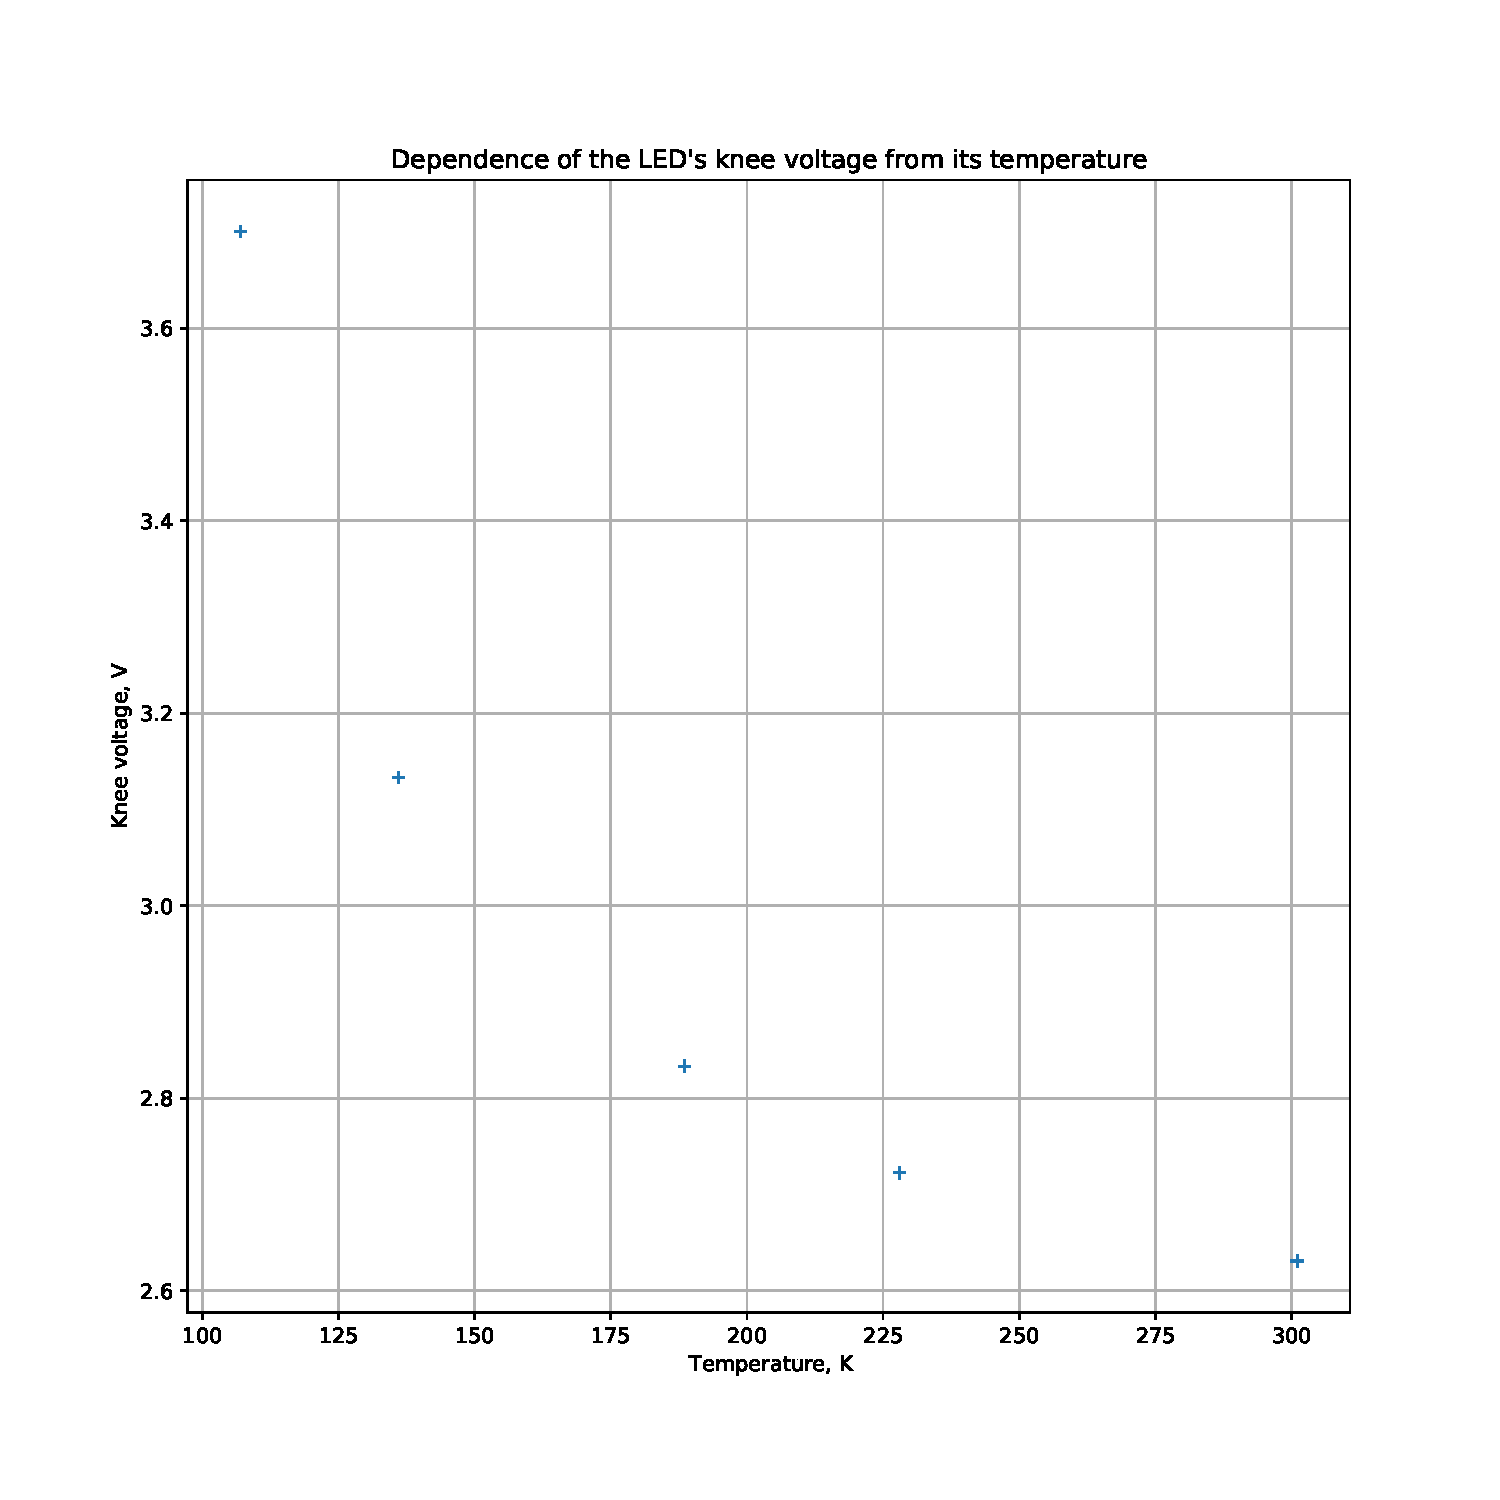
\includegraphics[width=\linewidth]{2_Knee_LED}
	\caption{Зависимость напряжения, при котором происходит ,,открытие'' светодиода, от его температуры.}
	\label{fig:2_Knee_LED}
\end{figure}

\subsection{Выводы}

\begin{enumerate}
	\item Была собрана экспериментальная установка для определения ВАХ диода и светодиода.
	
	\item Были получены экспериментальные зависимости формы ВАХ диода и светодиода от температуры.
	
	\item Были предложены зависимости $I_0$ от температуры для рассмотренных диода и светодиода на основании собранных экспериментальных данных.
\end{enumerate}

\newpage

\section{Изучение эффекта Холла}
\fancyhead[R]{\textsc{Изучение эффекта Холла}}%Вставить колонтитул сюда

\subsection{Цели работы}

\begin{enumerate}
	\item Пронаблюдать эффект Холла 
	
	\item Определить знак носителей заряда в полупроводнике 
	
	\item Определить подвижность и концентрацию носителей
	
	
\end{enumerate}
\subsection{Теория эффекта}
\subsubsection{Тензор сопротивления в магнитном поле}
Уравнение движения заряженной частицы, на которую действует электрическое поле в плоскости распространения заряда и магнитное поле перпендикулярно, можно записать как:
\begin{equation}
	m\frac{d\textbf{v}}{dt}=q(\textbf{E}+\textbf{v}\times\textbf{B})-m\frac{\textbf{v}}{\tau} \\
\end{equation}
Где \textbf{v} - средняя по всем частицам скорость. 

Подвижностью носителей заряда будет называться коэффициент пропорциональности между дрейфовой скоростью носителей и приложенным электрическим полем при отсутствии магнитного: $\mu$=q$\tau$/m

Тогда в стационарном состоянии d\textbf{v}/dt = 0 в матричном виде:

\begin{equation}
	\left(\begin{array}{ccc}
		1 & -\mu B & 0 \\
		\mu B & 1 & 0 \\
		0 & 0 & 1
	\end{array}\right)\left(\begin{array}{l}
		v_{x} \\
		v_{y} \\
		v_{z}
	\end{array}\right)=\mu\left(\begin{array}{l}
		E_{x} \\
		E_{y} \\
		E_{z}
	\end{array}\right)
\end{equation}
Вводя тензор сопротивления: $\textbf{E}=\hat{\rho} \textbf{j} = ne \hat{\rho}\textbf{v}$, где n - концентрация носителей заряда получаем:
\begin{equation}
	\hat{\rho}=\frac{1}{n e \mu}\left(\begin{array}{ccc}
		1 & -\mu B & 0 \\
		\mu B & 1 & 0 \\
		0 & 0 & 1
	\end{array}\right)
\end{equation}
И, соответственно, обратный тензор проводимости:
\begin{equation}
	\hat{\sigma}=\frac{\hat{\sigma}_{0}}{1+(\sigma B)^{2}}\left(\begin{array}{ccc}
		1 & \mu B & 0 \\
		-\mu B & 1 & 0 \\
		0 & 0 & 1
	\end{array}\right),
\end{equation}
где $\sigma_0=ne\mu$.

\subsubsection{Подвижность и концентрация носителей. Схема снятия снятия напряжений}
Изучаемый образец (\ref{fig:3_sample2}) представляет из себя узкий и длинный прямоугольный параллелепипед с известными геометрическими параметрами. Токовые контакты (1 и 4) находятся на торцах образца, и ток, соответственно течет вдоль продольного направления, а магнитное поле направлено ему перпендикулярно.

\begin{figure}[H]
	\centering
	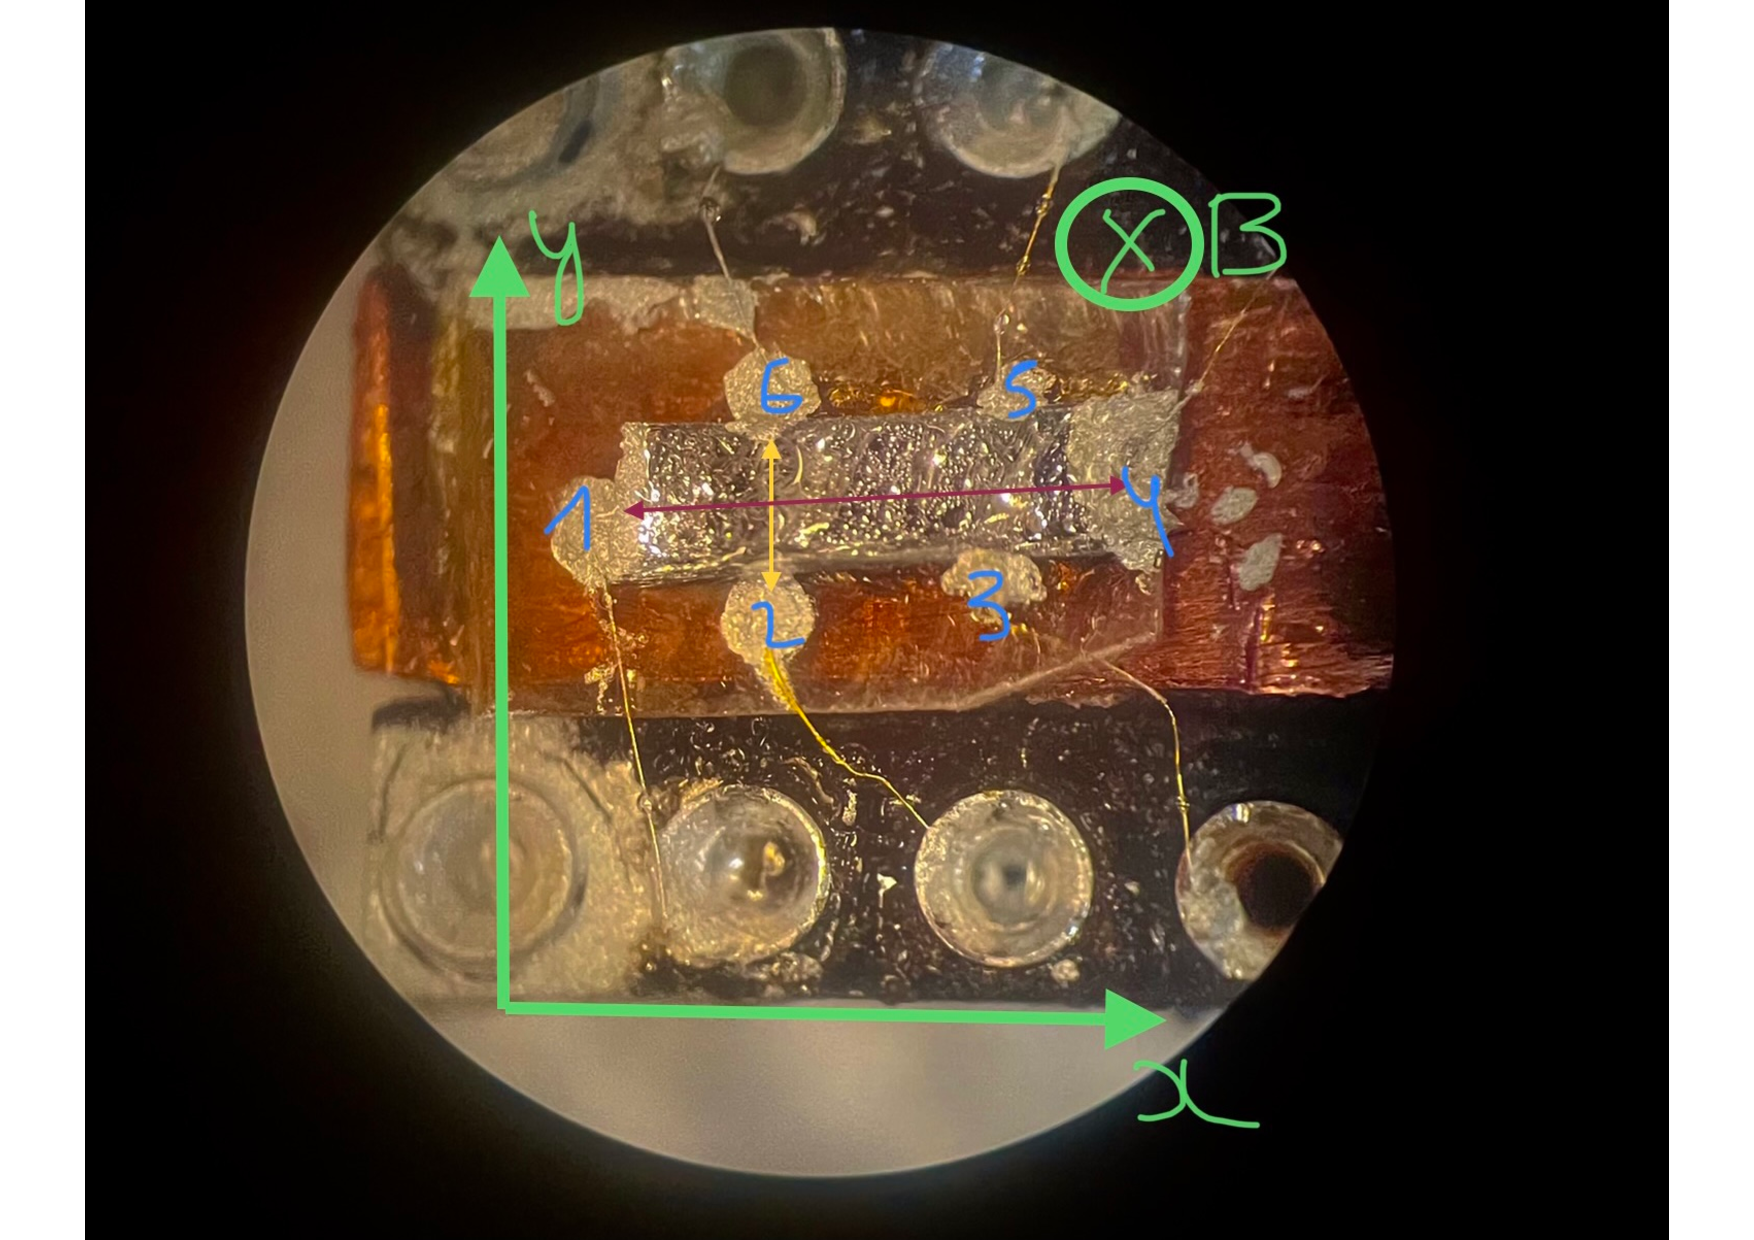
\includegraphics[width=\linewidth]{3_Sample2.pdf}
	\caption{Образец}
	\label{fig:3_sample2}
\end{figure}
Электроны под действием силы Лоренца будут отклоняться от направление тока и, соответственно, создавать разность потенциалов между краями образца (между 6 и 2, 5 и 3). То есть компонента электрического поля будет возрастать до тех пор, пока не компенсирует силу Лоренца. 

В установившемся состоянии тока вдоль оси y не будет, то есть: 
\begin{equation}
	\left(\begin{array}{c}
		j_x \\
		0
	\end{array}\right)=\frac{\hat{\sigma}_{0}}{1+(\mu B)^{2}}\left(\begin{array}{cc}
		1 & \mu B \\
		-\mu B & 1
	\end{array}\right)\left(\begin{array}{c}
		E_{x} \\
		E_{y}
	\end{array}\right)
\end{equation}
При этом $E_x=U_{xx}/l$ и $E_y=U_{xy}/w$, тогда
\begin{equation}
	\mu=\frac{1}{B}\frac{V_y}{V_x}\frac{l}{w}
\end{equation}
Также, зная направление тока и магнитного поля, а также знак холловского поперечного напряжения, можно определить тип носителей заряда, соответствующему знаку подвижности.

Записывая полный ток через образец, выразим его через концентрацию:
\begin{equation}
	I=j_xwh=(\sigma_{xx}E_x+\sigma_{xy}E_y)wh=\sigma_0 wh=ne\mu wh
\end{equation}
А следовательно
\begin{equation}
	n=\left(eh\frac{V_y}{IB}\right)^{-1}
\end{equation}

\subsection{Ход работы}

\subsubsection{Калибровка магнита}

Калибровка магнита с помощью теслометра позволила произвести взаимооднозначное соответствие силы подаваемого тока и напряженности поля внутри магнита. Также было установлено соответствие полярности подключения источника тока и направления поля. Результаты измерений приведены на графике (\ref{fig:3_calib}) Полученная зависимость: 26.2 mТл/А

\begin{figure}[H]
	\centering
	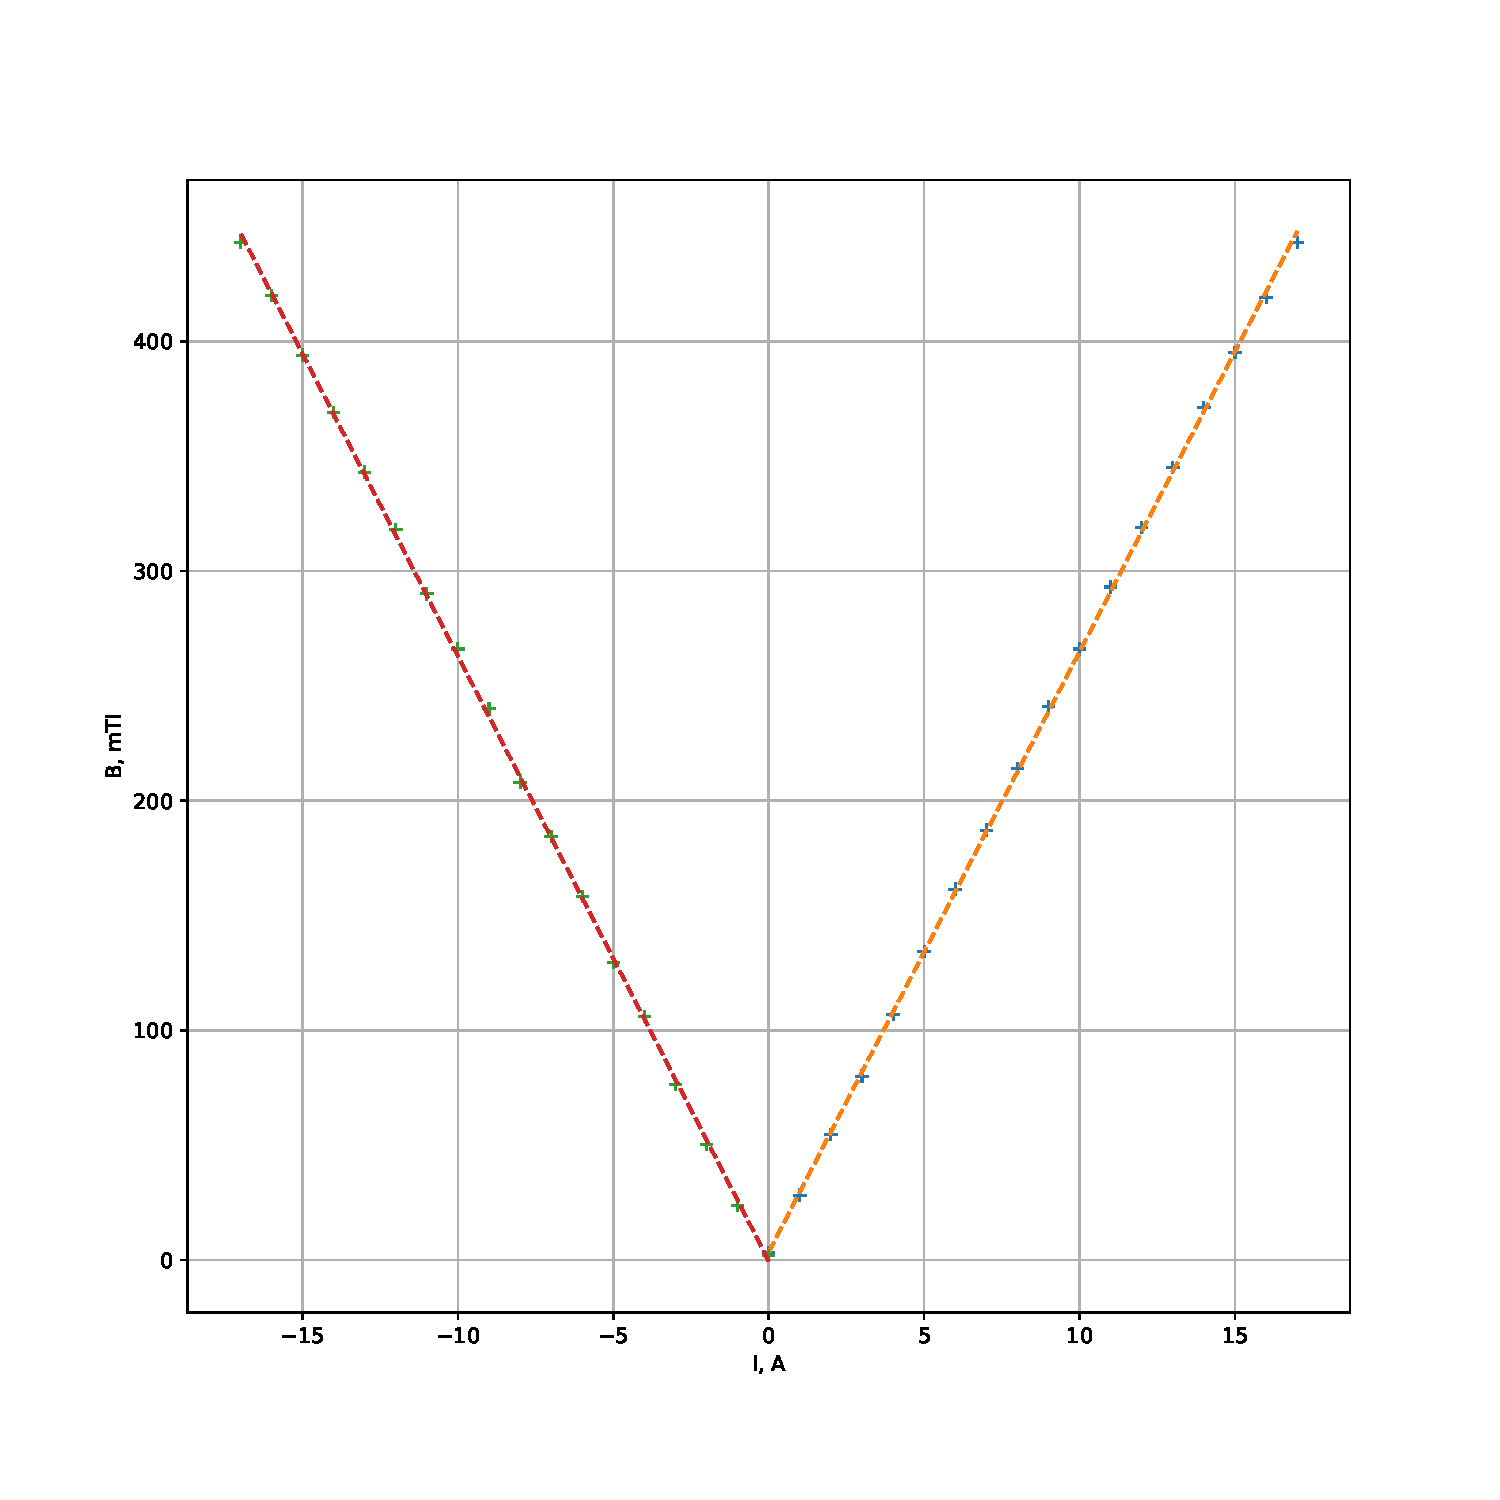
\includegraphics[width=0.7\linewidth]{3_Calibration.pdf}
	\caption{Зависимость напряженности поля от тока}
	\label{fig:3_calib}
\end{figure}

\subsubsection{Снятие данных зависимости продольного и поперечного напряжений от величины и направления магнитного поля }
Схема электрической цепи была собрана на вставке в криостат и разводящей коробке с общей землей, соединенной посредством внешним оплеток bnc-разъемов. Это позволяло легко переключаться между контактами для измерения продольного и поперечного  наряжений.

На встроенном в усилитель Lock-in генераторе было установлено напряжение 5 В, в цепь последовательно был подключен резистор сопротивлением 5.05 $k\Omega$. Это сопротивление много больше сопротивления на образце ($\approx$ 60 $\Omega$), а следовательно ток через полупроводник: $$I=5 \;V/5.05 \; k\Omega\approx 1\text{ mА}$$

Далее образец помещался в магнитное поле и снималась зависимость продольного и поперечного напряжений от велечины индукции магнитного поля. Аналогичный опыт проводился после погружения образца в азот и, соответственно его охлаждение до 77 K.

\subsection{Обработка данных}
\subsubsection{Определение типа носителей заряда}
Как уже было сказано выше, тип носителей заряда определяется знаком подвижности и, соответственно, направлением Холловского электрического поля. 

На практике это происходило так: в конфигурации, изображенной на рисунке (\ref{fig:3_sample2}) ток был направлен вдоль оси x, а магнитное поле ,,от нас''. Считывание напряжения выдавало разность потенциалов между контактами 2 и 6. Тогда в предположении, что носителями заряда являются электроны, на нижнем краю образца будет под действием силы Лоренца скапливаться отрицательный заряд, а на верхнем положительный. И соответственно мы будет считывать отрицательное напряжение. В действительности же, в данной конфигурации мы наблюдали положительную разность потенциалов между контактами, что напрямую свидетельствует о том, что носители заряда --- дырки.
\subsubsection{Продольное напряжение}

Зависимость продольного сопротивления для $T=77$ K (между контактами 6 и 5) представлено на рисунке (\ref{fig:3_long})

Теоретически, зависимости продольного сопротивления, а следовательно и напряжения, от величины магнитного поля наблюдаться не должно. И действительно, разброс снятых величин составляет порядка 1 процента. Эти флуктуации можно объяснить неидеальным расположением контактов относительно направления тока (то есть возникновение холловского напряжения), слабой точность позиционирования образца в магнитном поле и т.д. 

Значения измеренного продольного напряжения для комнатной температуры:
$$V_{xx} = 229 \; \mu \text{В}  $$

Для 77K:
$$V_{xx} = 17.46 \; \mu \text{В} $$

\begin{figure}[H]
	\centering
	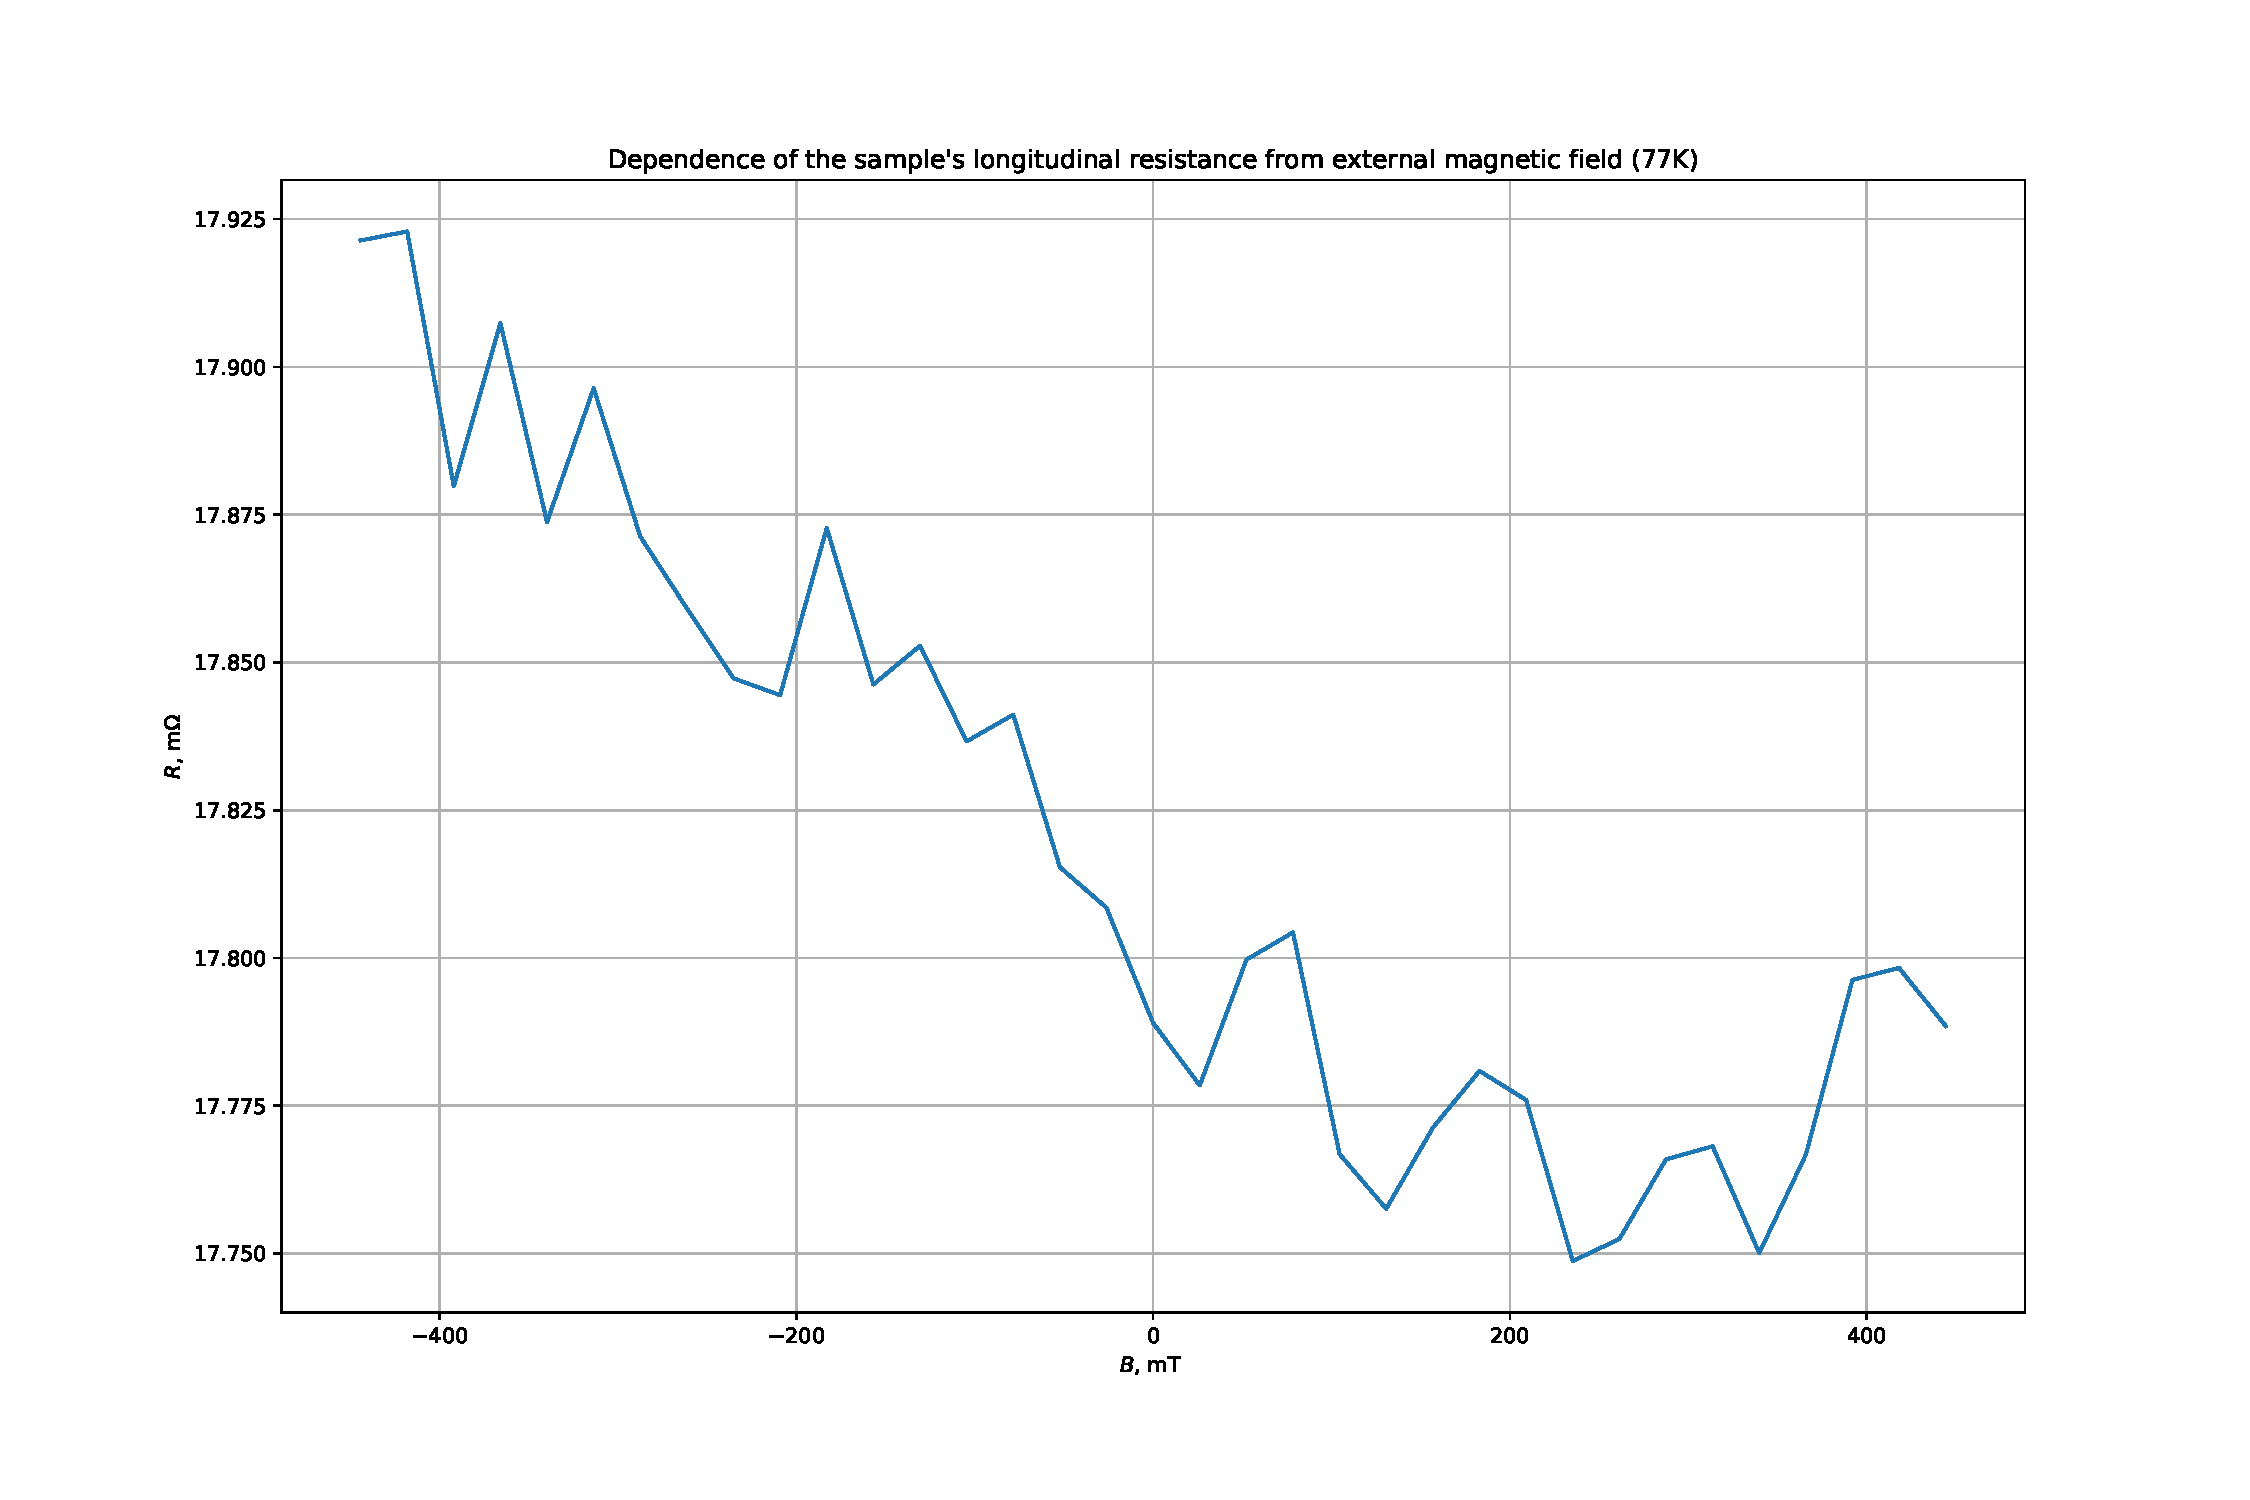
\includegraphics[width=\linewidth]{3_longitudunal.pdf}
	\caption{Зависимость продольного сопротивления от поля}
	\label{fig:3_long}
\end{figure}

\subsubsection{Поперечное сопротивление}

Данные зависимости Холловского сопротивления от величины индукции магнитного поля приведены на рисунке (\ref{fig:3_room}) для комнатной температуры и на рисунке (\ref{fig:3_cold}) для температуры азота.

Напомним формулы для подвижности носителей заряда и их концентрации:
$$\mu=\frac{1}{B}\frac{V_y}{V_x}\frac{l}{w}; \qquad n=\left(eh\frac{V_y}{IB}\right)^{-1}  $$
При этом $V_y/(IB) = R_y/B$ --- наклон прямой зависимости холловского сопротивления от магнитного поля. $h = 180$ $\mu$м --- толщина образца.

Таким образом концентрация носителей заряда при температуре 77 K:

$$n\approx15 \cdot 10^{19}\text{ см}^{-3}$$ 

При комнатной температуре:
$$n\approx21 \cdot 10^{19}\text{ см}^{-3}$$ 
\begin{figure}[H]
	\centering
	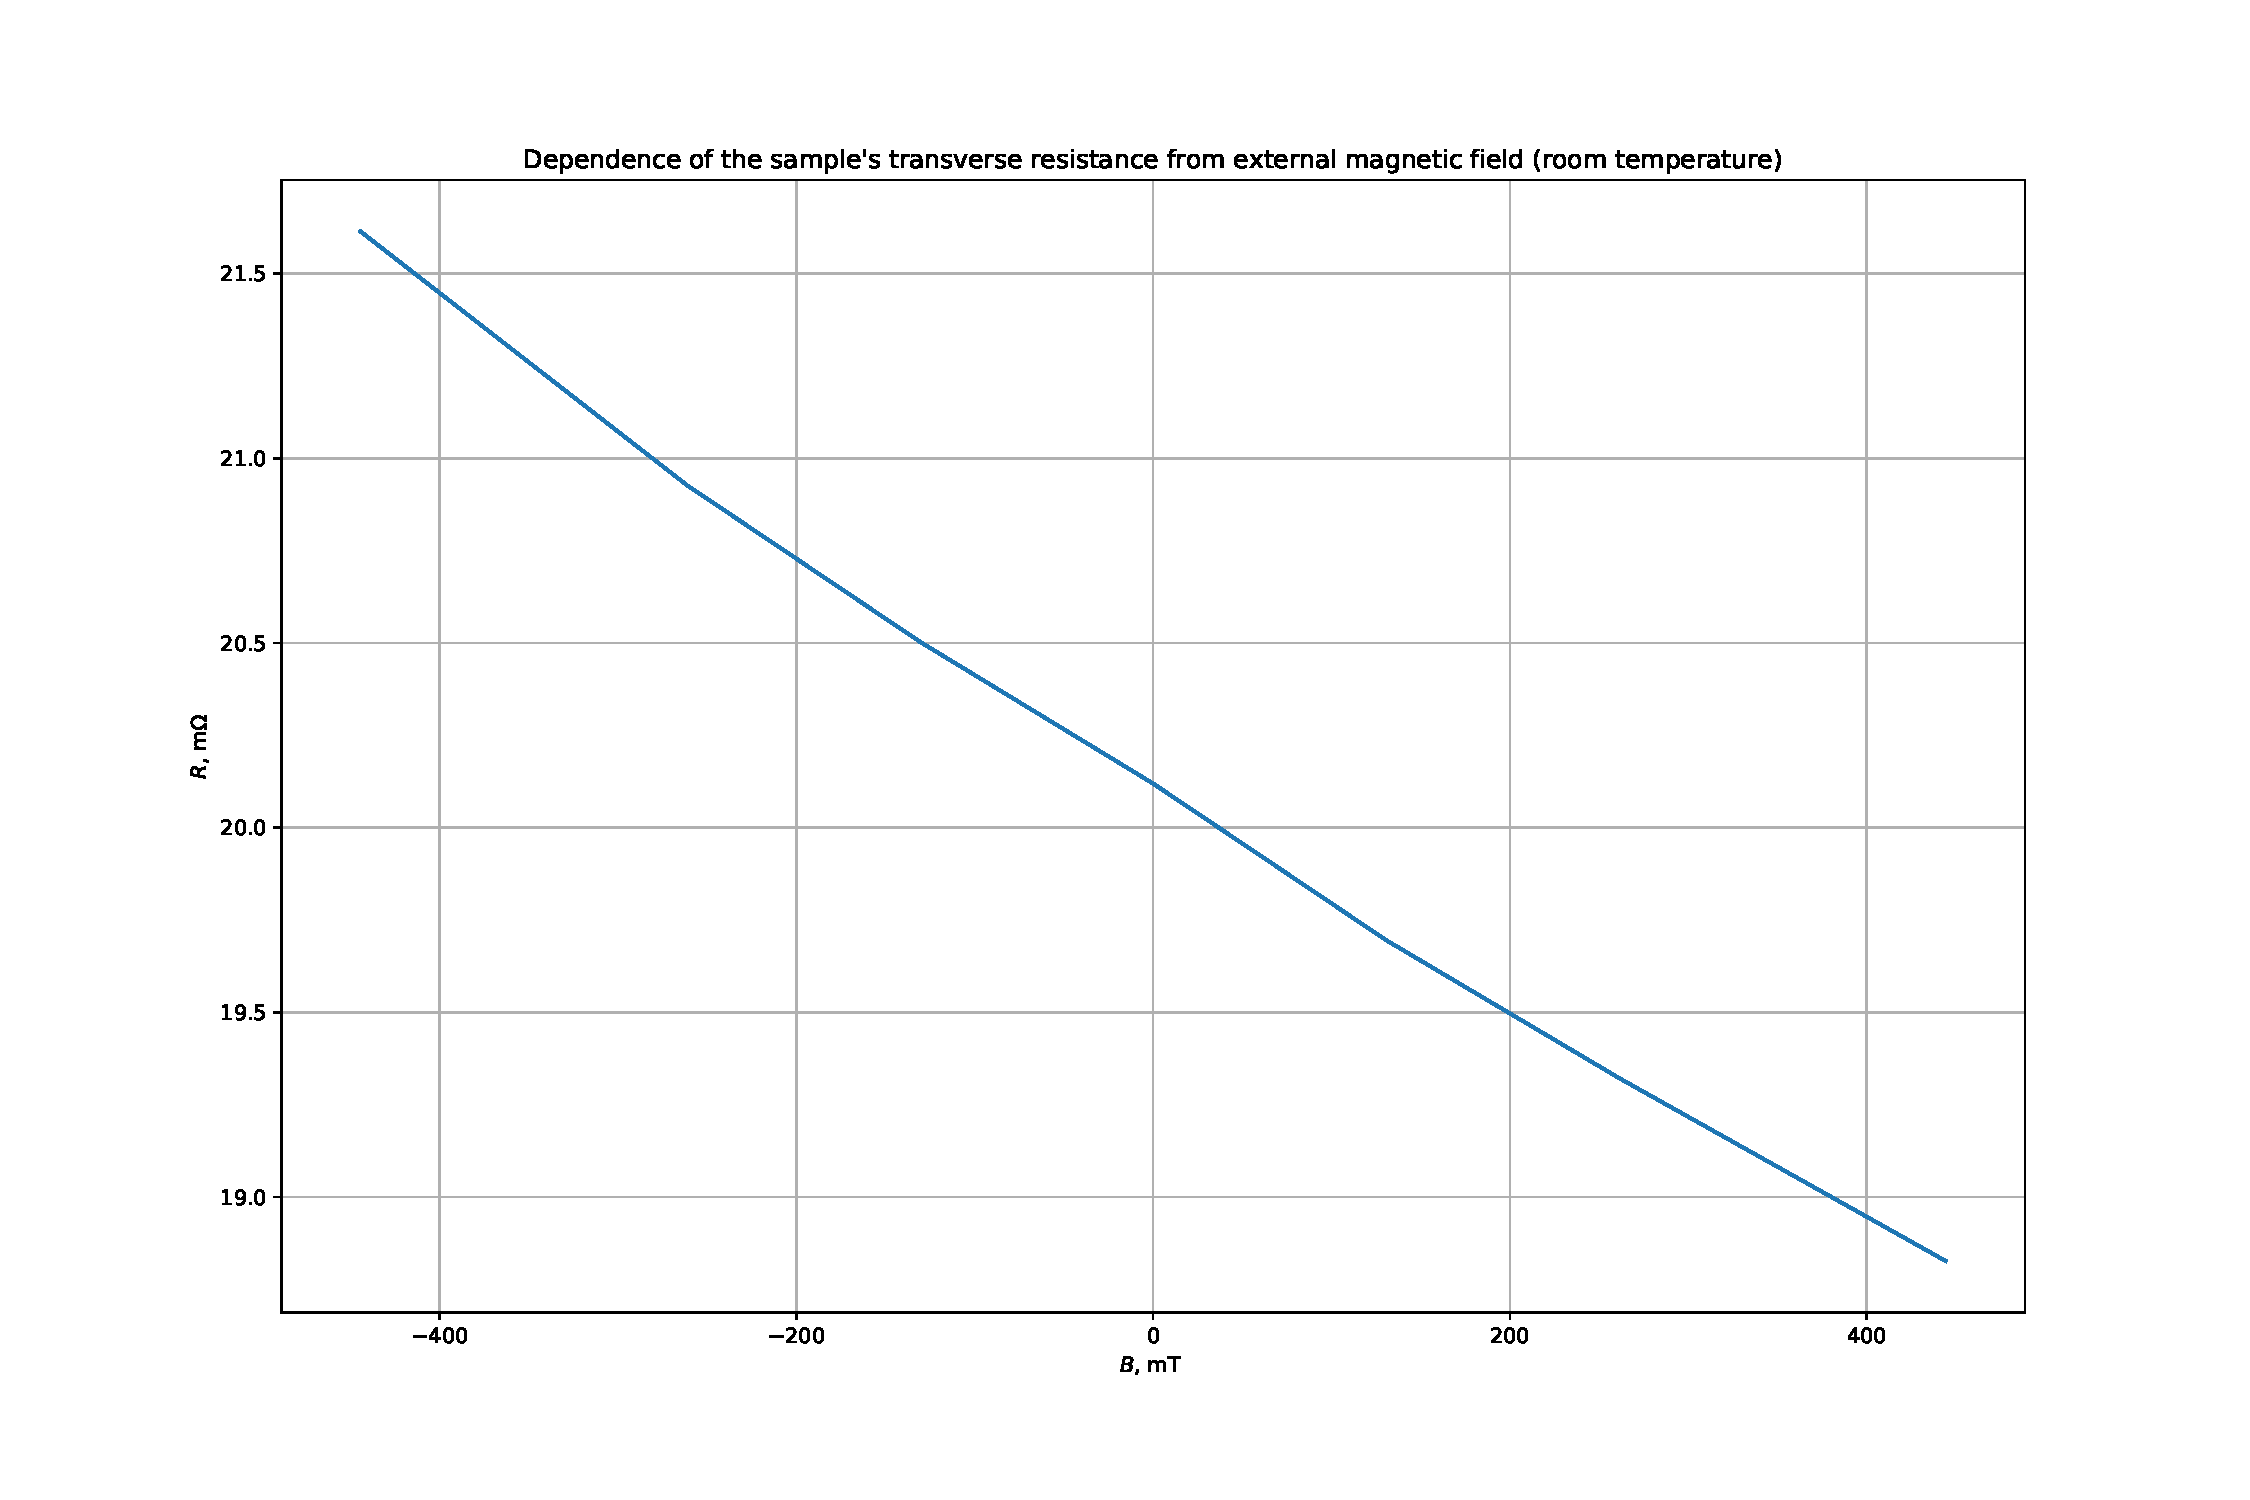
\includegraphics[width=0.8\linewidth]{3_room.pdf}
	\caption{Зависимость поперечного сопротивления от поля (комнатная температура)}
	\label{fig:3_room}
\end{figure}

\begin{figure}[H]
	\centering
	\includegraphics[width=0.8\linewidth]{3_cold.pdf}
	\caption{Зависимость поперечного  сопротивления от поля (температура жидкого азота)}
	\label{fig:3_cold}
\end{figure}

Измеряя отношение расстояний между продольными и поперечными контактами: $l_1$/$w$=1.7, находим значение подвижности при комнатной температуре:
$$\mu\approx 0.72  \; \frac{\text{м}^2}{\text{В} \cdot \text{с}}$$

И при 77 K:

$$\mu\approx 3.2   \; \frac{\text{м}^2}{\text{В} \cdot \text{с}}$$

Наблюдаемый эффект возникновения поперечного напряжения линеен по полю. При этом заметим, что при нулевой напряженности магнитного поля, вопреки теоретическому ожиданию, все равно существует ненулевое напряжение. Объясняется это, как уже было сказано выше, неточностью расположения контактов и рядом других факторов. 

Тогда симметризацией тензора напряжения и сопротивления мы получим постоянное значение, а антисимметризацией линейное по полю:

$$ \rho_{xx}=\frac{R(B)+R(-B)}{2};\quad \rho_{xy}=\frac{R(B)-R(-B)}{2}$$

Подставляя измеренные значения получаем для 298 K:

$$\rho_{xx}\approx 20.1 \text{ m$\Omega$}; \quad \rho_{xy}\approx0.00312B \text{ m$\Omega$}$$

И для 77 K:
$$\rho_{xx}\approx7.9 \text{ m$\Omega$}; \quad \rho_{xy}\approx0.00238B \text{ m$\Omega$}$$

Для корректности последних вычислений предлагается подставлять $B$ в mТл.

\subsection{Выводы}

\begin{enumerate}
	\item Было совершено наблюдение эффекта Холла.
	
	\item Было установлено, что носителями заряда являются дырки.
	
	\item Была определена подвижность (\mbox{$\mu\approx 0.72$~м$^2$/(В$\cdot$с)} при комнатной температуре и \mbox{$\mu \approx3.2$~м$^2$/(В$\cdot$с)} при 77 К), а также концентрация ($n\approx 15 \cdot 10^{19}$~см$^{-3}$ при комнатной температуре и $n\approx 21 \cdot 10^{19}$~см$^{-3}$ при 77 К).
	
	\item Были определены компоненты тензора сопротивления: $\rho_{xx}\approx 20.1 \text{ m$\Omega$}$, $\rho_{xy}\approx0.00312B \text{ m$\Omega$}$ при комнатной температуре; $\rho_{xx}\approx 7.9 \text{ m$\Omega$}$, $\rho_{xy}\approx0.00238B \text{ m$\Omega$}$ при 77 К. $B$ подставляется в зависимость в mТл.
\end{enumerate}

\newpage

\begin{thebibliography}{2}
	\bibitem{Glazkov}
	Глазков, В. Н. Лекция 7. Контактные явления в полупроводниках. Построение энергетических диаграмм контактов полупроводников. / В. Н. Глазков --- Москва : Московский физико-технический институт, Кафедра общей физики, 2016.
	
	\bibitem{Igoshin}
	Игошин Ф. Ф. Лабораторный практикум по общей физике. / Ф. Ф. Игошин, Ю. А. Самарский, Ю. М. Ципенюк ; под редакцией Ципенюка Ю. М. --- Москва : Физматкнига, 2005.
\end{thebibliography}

\end{document}